\documentclass[master=eelt,masteroption=em]{kulemt}
\setup{title={Practical Identity-Based Encryption for Online Social Networks},
  author={Stijn Meul},
  promotor={Prof.\,dr.\,ir.\ Bart Preneel \and Prof.\,dr.\,ir.\ Vincent Rijmen},
  assessor={Prof.\,dr.\,ir.\,Claudia Diaz\and Prof.\,dr.\,ir.\ Frank Piessens},
  assistant={Filipe Beato}}
% The following \setup may be removed entirely if no filing card is wanted
\setup{filingcard,
  translatedtitle=,
  udc=621.3,
  shortabstract={Here comes a very short abstract, containing no more than 500
    words. \LaTeX\ commands can be used here. Blank lines (or the command
    \texttt{\string\pa r}) are not allowed!
    \endgraf \lipsum[2]}}
% Uncomment the next line for generating the cover page
%\setup{coverpageonly}
% Uncomment the next \setup to generate only the first pages (e.g., if you
% are a Word user.
%\setup{frontpagesonly}

% Choose the main text font (e.g., Latin Modern)
\setup{font=lm}

% If you want to include other LaTeX packages, do it here. 

% Finally the hyperref package is used for pdf files.
% This can be commented out for printed versions.
\usepackage[pdfusetitle,plainpages=false]{hyperref}

\usepackage{kulemtx}
\headstyles{kulemtman}
%%%%%%
% Extra packages
\usepackage{amsthm}
\usepackage{amsfonts}
\usepackage{amsmath}
\usepackage{algorithm}
\usepackage{algpseudocode}
\usepackage{tikz}
\usepackage{caption}
\usepackage{transparent}
\usepackage{bbding}
\usepackage{afterpage}
\usetikzlibrary{arrows,positioning}

%%%%%%
% Make theorem titles bold
\makeatletter
\def\th@plain{%
  \thm@notefont{}% same as heading font
  \itshape % body font
}
\def\th@definition{%
  \thm@notefont{}% same as heading font
  \normalfont % body font
}
\makeatother

%%%%%%%
% The lipsum package is used to generate random text.
% You never need this in a real master thesis text!
\IfFileExists{lipsum.sty}%
 {\usepackage{lipsum}\setlipsumdefault{11-13}}%
 {\newcommand{\lipsum}[1][11-13]{\par And some text: lipsum ##1.\par}}
%%%%%%%
\newenvironment{game}
  {\begin{algorithm}\floatname{algorithm}{Game}
  }{\end{algorithm}}



% Reset theorem numbering for each chapter
\theoremstyle{plain}
\newtheorem{thm}{Theorem}[chapter]

% definition numbers are dependent on the theorem numbers
\theoremstyle{definition}
\newtheorem{defn}[thm]{Definition}

\newcommand{\id}[1]{\ensuremath{\mathtt{id}_{#1}}}

%\includeonly{chap-n}
\begin{document}
%TODO: vraag aan begeleider hoe Game opnieuw moet worden genummerd...

\begin{preface}
  I would like to thank everybody who kept me busy the last year,
  especially my promotor and my assistants. I would also like to thank the
  jury for reading the text. My sincere gratitude also goes to my wive and
  the rest of my family.
\end{preface}

\tableofcontents*

\begin{abstract}
  The \texttt{abstract} environment contains a more extensive overview of
  the work. But it should be limited to one page.

  \lipsum[1]
\end{abstract}

% A list of figures and tables is optional
%\listoffigures
%\listoftables
% If you only have a few figures and tables you can use the following instead
\listoffiguresandtables
% The list of symbols is also optional.
% This list must be created manually, e.g., as follows:
\chapter{List of Abbreviations}
\begin{flushleft}
  \renewcommand{\arraystretch}{1.1}
  \begin{tabularx}{\textwidth}{@{}p{30mm}X@{}}
    IBE   & Identity-Based Encryption \\
    PKG   & Public Key Generator \\
    DKG   & Distributed Key Generator \\
    IND-CPA  & Indistinguishability under Chosen Plaintext Attack  \\
    IND-CCA & Indistinguishability under Chosen Ciphertext Attack \\
    ANO-IBE & Anonymous IBE \\
    ANO-IND-CPA & Anonymity preserving IBE scheme that is indistinguishable under chosen plaintext attacks \\
    ANO-IND-CCA & Anonymity preserving IBE scheme that is indistinguishable under chosen ciphertext attacks \\ 
    OSN & Online Social Network \\
  \end{tabularx}
\end{flushleft}
\chapter{List of Symbols}
\begin{flushleft}
 \renewcommand{\arraystretch}{1.1}
 \begin{tabularx}{\textwidth}{@{}p{30mm}X@{}}
  $\lambda$ & Security parameter \\
  $l$ & The number of bits required to realise security level $\lambda$ \\
  $s$ & Secret \\
  $sk_i$ & Private key corresponding to the public key $pk_i$ or the public verifying key $vk_i$ depending on the application \\
  $pk_i$ & Public key with corresponding private key $sk_i$ \\
  $vk_i$ & Verifying key with corresponding signing key $sk_i$ \\
  $\{ 0,1 \}^l$ & Binary bit sequence of length $l$ \\
  $\{ 0,1 \}^*$ & Binary bit sequence of variable length \\
  $m$ & Message \\
  $c$ & Ciphertext \\
  $v, w$ & Binary bit sequences \\
  $\{ v \parallel w \}$ & Concatenated bit sequences \\
  \id{Alice} & Identity of Alice \\ 
  $s_{\id{Alice}}$ & IBE private key corresponding to the identifier \id{Alice} \\
  $k$ & Generic symmetric session key \\
  $E_k \left( m \right)$ & Symmetric encryption of the message $m$ under session key $k$ \\
  $D_k \left( c \right)$ & Symmetric decryption of the ciphertext $c$ under session key $k$ \\
  $G$ & Group $\left( G, * \right)$ \\
  $S_A \left( m \right)$ & Signature of entity $A$ on message $m$ \\
  $S_{sk_A} \left( m \right)$ & Signature generated by the signing key $sk_A$ of entity $A$ on message $m$ \\
  $e: G_1 \times G_2 \rightarrow G_T$ & Bilinear map \\
  $U, P, Q$ & Points on an elliptic curve \\
  $e \left( P, Q \right)$ & Bilinear map  for the points $P \in G_1, Q \in G_2$ such that $e \left( P, Q \right) \in G_T$ \\  
  $\mathcal{A} \left( a, b \right)$ & Algorithm $\mathcal{A}$ with parameters $a$ and $b$ \\
  $\left< a, b, c \right> \leftarrow \mathcal{A}( d, e )$ & Algorithm $\mathcal{A}$ with parameters $d$ and $e$, returns the collection of values $a, b, c$ \\
  \end{tabularx}
\end{flushleft}

% Now comes the main text
\mainmatter

\chapter{Introduction}
\label{cha:intro}
The newest internet trend at the dawn of the 21st century certainly is the Online Social Network (OSN). Words like tweeting, sharing, liking, trending and tagging have found common acceptance in the vocabulary of today's internet savvy users while services like Facebook, Google+, LinkedIn and Twitter have become part of everyday life. 

The far reaching influence of today's most popular OSNs is best illustrated with the help of some statistics. In May 2013, 72\% of all internet users were active on a social network~\cite{site:Jones13}. At the time of writing, Facebook has 1.23 Billion monthly active users which corresponds to 17\% of the global population~\cite{site:Bullas14,site:worldometers}. Furthermore, the average Facebook user spends 15 hours and 33 minutes online per month~\cite{site:StatisticBrain}. These numbers show that social networks no longer represent the latest craze of an internet bubble but are conversely deeply rooted in our daily habits.



\section{Problem Statement}

\section{Previous Work}

\section{Goals of this Thesis}

\section{Structure of this Thesis}

%%% Local Variables: 
%%% mode: latex
%%% TeX-master: "thesis"
%%% End: 

\chapter{Preliminaries}
\label{cha:1}
This chapter covers briefly the mathematical knowledge required to understand the mechanics behind cryptographic algorithms presented later in this text. First, next, then, finally,... %TODO: verder aanvullen hoe de structuur van dit hoofdstuk eruit gaat zien

Note that this chapter only scratches the surface of cryptographic fundamentals to understand the remainder of the thesis. Definitions are always provided without proof. For a more in depth discussion about the topics in this chapter, the reader is refered to~\cite{book:handbook_of_applied_cryptography} and~\cite{book:survey_of_modern_algebra}.

If the reader feels he has sufficient background of the concepts covered in this chapter, the chapter can be skipped without loss of comprehension.

\section{Complexity Theory}

In practice no modern cryptographic agorithm achieves perfect secrecy\footnote{Note that the one-time pad is not taken into account. Although it is the only proven information secure cryptographic algorithm, it is seldom used in practical cryptographic systems.}, i.e. with unbounded computational power all practical cryptographic algorithms can be broken. Therefore a more pragmatic definition of security is always considered, namely security against adversaries that are computationally bound to their finite resources. In this pragmatic view of security an algorithm is considered secure only if the probability of success is smaller than the reciprocal of any polynomial function. The negligible function can be used to exactly describe this notion in a formal way.

\begin{defn}
\label{def:negligible_function}
A \textbf{negligible function} in $k$ is a function $\mu \left( k \right): \mathbb{N} \rightarrow \mathbb{R}$ if for every polynomial $p \left( . \right)$ there exists an $N$ such that for all $k > N$~\cite{book:Goldreich97}
 \begin{equation*}
  \mu \left( k \right) < \frac{1}{p\left( k \right)} 
 \end{equation*}
\end{defn}

The negligible function will be used later on in this chapter to formally describe computationally infeasible problems. In such a context $k$ often represents the security parameter. The larger $k$ will be chosen, the smaller $\mu \left( k \right)$ will be.

\section{Abstract Algebra}
Abstract algebra is a field of mathematics that studies algebraic structures such as groups, rings and vector spaces. These algebraic structures define a collection of requirements on mathematical sets such as e.g., the natural numbers $\mathbb{N}$ or matrices of dimension 2 x 2 $\mathbb{R}^{2 x 2}$. If these requirements hold, abstract properties can be derived. Once a mathematical set is then categorised as the correct algebraic structure, properties derived for the algebraic structure will hold for the set as a whole.

In the light of our further discussion, especially additive and multiplicative groups prove to be essential concepts. However, algebraic groups come with a specific vocabulary such as binary operation, group order and cyclic group that are defined in this section as well.

\begin{defn}[Binary operation]
 A \textit{binary operation} * on a set $S$ is a mapping $S \times S \rightarrow S$. That is, a binary operation is a rule which assigns to each ordered pair of elements $a$ and $b$ from $S$ a uniquely defined third element $c = a*b$ in the same set $S$.~\cite{book:handbook_of_applied_cryptography,book:survey_of_modern_algebra}
\end{defn}

\begin{defn}[Group]
\label{def:group}
 A \textit{group} $\left( G, * \right)$ consists of a set $G$ with a binary operation $*$ on $G$ satisfying the following three axioms:
 \begin{enumerate}
  \item \textit{Associativity} $\forall a, b, c \in G: a*(b*c) = (a*b)*c$
  \item \textit{Identity element} $\forall a \in G, \exists e \in G: a*e = e*a = a $ where $e$ denotes the \textit{identity element} of $G$
  \item \textit{Inverse element} $\forall a \in G, \exists a^{-1}: a*a^{-1} = a^{-1}*a = 1$ where $a^{-1}$ denotes the \textit{inverse element} of $a$
  \newcounter{enumTemp}
  \setcounter{enumTemp}{\theenumi}
 \end{enumerate}

\end{defn}

\begin{defn}[Commutative group]
 A group $\left( G, * \right)$ is called a \textit{commutative group} or an \textit{abelian group} if in addition to the properties in Definition~\ref{def:group}, also commutativity holds.
 \begin{enumerate}
  \setcounter{enumi}{\theenumTemp}
  \item \textbf{Commutativity} $\forall a, b \in G: a*b = b*a$
 \end{enumerate}

\end{defn}

From here on a group $\left( G, * \right)$ will be denoted $\mathbb{G}$. Depending on the group operation~$*$, $\mathbb{G}$ is called either a \textit{multiplicative group} or an \textit{additive group}. In Definition~\ref{def:group} the multiplicative notation is used. For an additive group  the inverse of $a$ is often denoted $-a$~\cite{book:handbook_of_applied_cryptography}.

The perfect example of a commutative group is the set of integers with the addition operation $\left( \mathbb{Z}, + \right)$ since the addition is both associative and commutative in $\mathbb{Z}$. Furthermore, the identity element $e = 0$ and the inverse element $\forall a \in \mathbb{Z}$ is $-a \in \mathbb{Z}$. Note that the set of natural numbers with the addition operation $\left( \mathbb{N}, + \right)$ is not a commutative group because not each element of $\mathbb{N}$ has an inverse element.

\begin{defn}[Cyclic group]
\label{def:cyclic_group}
 A group $\mathbb{G}$ is \textit{cyclic} if and only if $\forall b \in \mathbb{G}, \exists g \in \mathbb{G},\exists n \in \mathbb{Z}: g^n = b$. Such an element $g$ is called a \textbf{generator} of $\mathbb{G}$.
\end{defn}

Definition~\ref{def:cyclic_group} implies that in a cyclic group every element can be written as a power of one of the group's generators.

\begin{defn}[Finite group]
\label{def:finite_group}
 A group $\mathbb{G}$ is \textit{finite} if the number of elements in $\mathbb{G}$ denoted $|\mathbb{G}|$ is finite. The number of elements $|\mathbb{G}|$ in a finite group is called the \textit{group order}.
\end{defn}

The set $\mathbb{Z}_n$ denotes the set of integers modulo $n$. The set $\mathbb{Z}_5$ with the addition operation is a cyclic finite group of order 5. The set $\mathbb{Z}_5 \backslash \{0\}$ with the multiplication operation, often denoted $\mathbb{Z}^{*}_5$, is a cyclic finite group of order 4 where the neutral element $e=1$. Two is an example of a generator in $\mathbb{Z}^{*}_5$ since every element in $\mathbb{Z}^{*}_5$ can be written as $\{ 2^n | n \in \mathbb{Z} \}$.

\begin{defn}[Order of an element]
\label{def:order_of_an_element}
Let $\mathbb{G}$ be a group. The \textit{order of an element} $a \in G$ is defined as the least positive integer $t$ such that $a^t = e$. If there exists no such $t$, $t$ is defined as~$\infty$.
\end{defn}

\begin{thm}
\label{the:group_modulo_a_prime}
If the order of a group $G$ equals a prime $p$, the group is cyclic and commutative.
\end{thm}


\section{Number Theoretic Assumptions}

This section presents a collection of number theoretic assumptions. The security of our future constructions falls or stands on these assumptions. If one of these assumptions would prove to be invalid, not only this thesis would be superfluous, society would no longer be protected by cryptographic protocols like RSA or ElGamal encryption~\cite{art:Boneh98,book:handbook_of_applied_cryptography}.

In the definitions that follow $\left< G, n, g \right> \leftarrow \mathcal{G} \left( 1^k \right)$ is defined as the setup algorithm that generates a group $G$ of order $n$, a generator $g \in G$ and an element $a \in G$ on input of the security parameter $k$.

\begin{defn}[DL]
\label{def:dl}
The \textit{discrete logarithm problem} is defined as follows. Given a finite cyclic group $G$ of order $n$, a generator $g \in G$ and an element $a \in G$, find the integer $x, 0 \leq x \leq n-1$ such that $g^x = a$.

The \textit{discrete logarithm assumption} holds if for any algorithm $\mathcal{A} \left( g, g^x \right)$ trying to solve the DL problem there exists a negligible function $\mu \left( k \right)$ such that 
 \begin{equation*}
  \textrm{Pr} \left[ \mathcal{A} \left( g, g^x \right) = a \mid \left< G, n, g \right> \leftarrow \mathcal{G} \left( 1^{k} \right)\right] \leq \mu \left( k \right)
 \end{equation*}
 where the probability is over the random choice of $n, g$ in $G$ according to the distribution induced by $\mathcal{G} \left( 1^k \right)$, the random choice of $a$ in $G$ and the random bits of the algorithm $\mathcal{A}$.
\end{defn}


\begin{defn}[CDH]
\label{def:cdh}
The \textit{Computational Diffie-Hellman problem} is defined as follows. Given a finite cyclic group $G$ of order $n$, a generator $g \in G$ and $g^a, g^b$ with uniformly chosen random independent elements $a, b \in \{ 1, \ldots, | G |\}$ , find the value $g^{ab}$.


The \textit{Computational Diffie-Hellman assumption} holds if for any algorithm $\mathcal{A} \left( g, g^a, g^b \right)$ trying to solve the CDH problem there exists a negligible function $\mu \left( k \right)$ such that 
 \begin{equation*}
  \textrm{Pr} \left[ \mathcal{A} \left( g, g^a, g^b \right) = g^{ab} \mid \left< G, n, g \right> \leftarrow \mathcal{G} \left( 1^{k} \right)\right] \leq \mu \left( k \right)
 \end{equation*}
 where the probability is over the random choice of $n, g$ in $G$ according to the distribution induced by $\mathcal{G} \left( 1^k \right)$, the random choice of $a, b$ in $\{ 1, \ldots, | G |\}$ and the random bits of the algorithm $\mathcal{A}$.
\end{defn}

\begin{defn}[DDH]
\label{def:ddh}
The \textit{Decisional Diffie-Hellman problem} is defined as follows. Given a finite cyclic group $G$ of order $n$, a generator $g \in G$ and $g^a, g^b, g^{ab}, g^c$ with uniformly chosen random independent elements $a, b, c \in \{ 1, \ldots, | G |\}$, distinguish $\left< g, g^a, g^b, g^{ab} \right>$ from $\left< g, g^a, g^b, g^c \right>$.

Define $\mathcal{A} \left( x \right)$ as an algorithm returning \texttt{true} if $x = \left< g, g^a, g^b, g^{ab} \right>$ and \texttt{false} if $x = \left< g, g^a, g^b, g^c \right>$ for $c \neq ab$. The \textit{Decisional Diffie-Hellman assumption} holds if for any such algorithm $\mathcal{A} \left( x \right)$ there exists a negligible function $\mu \left( k \right)$ such that 
 \begin{equation*}
  \lvert \textrm{Pr} \left[ \mathcal{A} \left( \left< g, g^a, g^b, g^{ab} \right> \right) = \texttt{true} \right] - \textrm{Pr} \left[ \mathcal{A} \left( \left< g, g^a, g^b, g^{c} \right> \right) = \texttt{true} \right] \rvert \leq \mu \left( k \right)
 \end{equation*}
 where the probability is over the random choice of $n, g$ in $G$ according to the distribution induced by $\mathcal{G} \left( 1^k \right)$, the random choice of $a, b, c$ in $\{ 1, \ldots, | G | \} $ and the random bits of the algorithm $\mathcal{A}$.
\end{defn}


Definition~\ref{def:ddh} states that $\left< g, g^a, g^b, g^{ab} \right>$ and $\left< g, g^a, g^b, g^{c} \right>$ are \textit{computationally indistinguishable}. It means that no efficient algorithm exists that can distinguish both arguments with non-negligible probability. The concept of computational indistinguishable arguments bears close resemblance to statiscally indistinguishable ensembles. The reader is refered to~\cite{art:Goldwasser84} and~\cite{art:Goldwasser89} for a more in depth discussion of the topic. The intuitive interpretation of Definition~\ref{def:ddh} is that $g^{ab}$ looks like any other random element in $G$.

Someone with the ability to calculate discrete logarithms could trivially solve the CDH problem. That is, if $a$ and $b$ can be derived only from $\left< g^a, g^b \right>$, it becomes easy to calculate $g^{ab}$. Therefore, a group structure where the CDH assumption holds, immediately implies a group where the DL assumption is valid as well. There is no mathematical proof that supports the inverse relation. Thus, a group where the DL problem is hard not necessarily implies the CDH problem. For specific group structures~\cite{art:MaurerW98} and~\cite{art:MaurerW99} show that CDH immediately follows from the DL assumption, however, their proof can not be generalised to just any group.

There exists a similar relation between the CDH and the DDH problem. If a powerful algorithm could solve CDH, i.e. derive $g^{ab}$ from $\left< g, g^a, g^b \right>$ alone, it would become trivial to distinguish $\left< g, g^a, g^b, g^{ab} \right>$ from $\left< g, g^a, g^b, g^c \right>$. Again, an inverse relation can not be proven. As a matter of fact, concrete examples of groups exist where CDH is hard although DDH is not.

Therefore, the relation between DL, CDH and DDH is often written as follows
\begin{equation*}
 DDH \Rightarrow CDH \Rightarrow DL
\end{equation*}
The $\Rightarrow$ notation is then translated into "immediately implies". In a group where DDH is hard both CDH and DL will be hard. On the contrary, there exist group structures where the CDH and the DL assumption hold while DDH can be found easily. Such groups are called \textit{Gap Diffie-Hellman Groups}.

\begin{defn}[GDH]
\label{def:gdh}
The \textit{Gap Diffie-Hellman problem} is defined as follows. Solve the CDH problem with the help of a DDH oracle. Given a finite cyclic group $G$ of order $n$, a generator $g \in G$ and $g^a, g^b$ with uniformly chosen random independent elements $a, b \in \{ 1, \ldots, | G |\}$ , find the value $g^{ab}$ with the help of a DDH oracle $\mathcal{DDH} \left( g, g^a, g^b, z \right)$. Where the DDH oracle $\mathcal{DDH} \left( g, g^a, g^b, z \right)$ is defined to return \texttt{true} if $z = g^{ab}$ and \texttt{false} if $z \neq g^{ab}$.

The \textit{Gap Diffie-Hellman assumption} holds if for any algorithm $\mathcal{A} \left( g, g^a, g^b \right)$ trying to solve the CDH problem with the help of a DDH oracle $\mathcal{DDH} \left( g, g^a, g^b, z \right)$ there exists a negligible function $\mu \left( k \right)$ such that 
 \begin{equation*}
  \textrm{Pr} \left[ \mathcal{A} \left( g, g^a, g^b \right) = g^{ab} \mid \left< G, n, g \right> \leftarrow \mathcal{G} \left( 1^{k} \right)\right] \leq \mu \left( k \right)
 \end{equation*}
 where the probability is over the random choice of $n, g$ in $G$ according to the distribution induced by $\mathcal{G} \left( 1^k \right)$, the random choice of $a, b$ in $\{ 1, \ldots, | G |\}$ and the random bits of the algorithm $\mathcal{A}$.
\end{defn}

As discussed in the next Section~\ref{sec:bilinear_map} bilinear pairings are an example of a practical usable DDH oracle~\cite{art:JouxN03}.

\section{Bilinear Maps}
\label{sec:bilinear_map}

\subsection{Definition}

\begin{defn}[Admissible bilinear map]
 Let $G_1, G_2$ and $G_T$ be three groups of order $q$ for some large $q$. An \textit{admissible bilinear map} $e: G_1 \times G_2 \rightarrow G_T$ is defined as a map from the gap groups $G_1$ and $G_2$ to the target group $G_T$ that satisfies the following properties:
 \begin{enumerate}
  \item \textit{Bilinearity} $\forall a, b \in \mathbb{Z}, \forall g_1 \in G_1, \forall g_2 \in G_2: e \left( g_1^a, g_2^b \right) = e \left( g_1, g_2 \right)^{ab}$
  \item \textit{Non-degeneracy} If $g_1$ is a generator of $G_1$ and $g_2$ is a generator of $G_2$, $e \left( g_1, g_2 \right)$ is a generator of $G_T$
  \item \textit{Computability} There is an efficient algorithm to compute $e \left( g_1, g_2 \right)$ for all $g_1 \in G_1$ and $g_2 \in G_2$
 \end{enumerate}

\end{defn}


\subsection{Bilinear Diffie-Hellman Assumption}

\subsection{Variants of the Bilinear Diffie-Hellman Assumption}

\section{Secret Sharing}

\subsection{Definition}

\subsection{Verifiable Secret Sharing}

\section{Hash Functions}

\subsection{Definition}

\subsection{Standard Model}

\subsection{Random Oracle Assumption}

\section{Conclusion}
The final section of the chapter gives an overview of the important results
of this chapter. This implies that the introductory chapter and the
concluding chapter don't need a conclusion.

\lipsum[66]

%%% Local Variables: 
%%% mode: latex
%%% TeX-master: "thesis"
%%% End: 

\chapter{Literature Review}
\label{cha:2}

\section{Cryptology}
Cryptology is the science describing how to hide confidential information. Cryptology consists of two complementary fields that continuously try to outwit each other: cryptography and cryptanalysis. On the one hand, cryptography is the practice and study of techniques trying to hide information from undesired third parties. On the other hand, cryptanalysis is the domain of cryptology trying to derive information from hidden data.

\subsection{Symmetric Cryptography}
Figure~\ref{fig:cryptosystem} shows a typical cryptographic system often shortened to "cryptosystem". In a typical cryptosystem one party (often called Alice) tries to send a message $m$ over an insecure channel to another party (often called Bob). The channel is insecure as third parties like Eve can eavesdrop on the channel to read out data that is being sent over.

\begin{figure}
 \includegraphics[trim=40mm 120mm 40mm 120mm, clip]{img/cryptosystem.pdf}
 \caption{A cryptosystem~\cite{thesis:Wyseur09}}
 \label{fig:cryptosystem}
\end{figure}

\subsubsection{Confidentiality}
Figure~\ref{fig:cryptosystem} achieves confidentiality, i.e. the information in $m$ is protected from disclosure to unauthorised parties. To prevent eavesdroppers from reading out the message $m$, Alice and Bob have agreed on a key $k$ that is unknown to the outside world. Before sending a message $m$ over the insecure channel, Alice encrypts the message $m$ to a ciphertext $c$ under the secret key $k$ using an encryption algorithm $E_k$ such that $c = E_k \left( m \right)$. Ideally $c$ looks like random gibberish to eavesdroppers like Eve. Bob can then read out the original plaintext message $m$ by applying the decryption algorithm $D_k$ under the same key $k$. Cryptosystems as the one described in Figure~\ref{fig:cryptosystem} are called \textit{symmetric} as both Alice and Bob have to use the same key $k$ for encryption and decryption. 

Most cryptosystems that are practically used today satisfy Kerchoff's principle. Kerchoff's principle states that although the encryption and decryption mechanism are known to the outside world, the cryptosystem assures confidentiality as long as the symmetric key $k$ remains secret.

\subsubsection{One-time Pad}
A simple symmetric encryption algorithm $E_k$ could be to XOR the binary message $m$ with a binary key $k$ such that the ciphertext is equal to $c = m \oplus k$. Decryption $D_k$ would then consist of an XOR operation with the same binary symmetric key $k$ such that $m = c \oplus k = \left( m \oplus k \right) \oplus k$.  In such a scheme, the key $k$ should be a random binary string with the same length as the plaintext message $m$. This scheme was originally proposed by Vernam and is therefore often called the \textit{Vernam scheme}.

Further research on the Vernam scheme by Mauborgne showed that the Vernam scheme can be proven information theoretic secure if $k$ is chosen completely random and used only once. Because of these requirements on the key $k$, the Vernam scheme is more widely known as the \textit{one-time pad}.

\subsubsection{Practical Encryption Algorithms}
Because the one-time pad is proven information theoretic secure, it can not be broken even if the adversary has access to unlimited computing power. Although this is a desirable property, the one-time pad is not frequently used in modern cryptosystems due to its impractical key management.

Suppose Alice and Bob have a lot of secret information to share. This would require that the a priori agreed key $k$ is long enough to hide all this information. Once the size of the message $m$ becomes larger than the key $k$, Alice and Bob should agree on new random bits in $k$ to secure the remainder of their conversation. In fact, they have to agree upfront on as much random bits in $k$ as there will be bits in the message $m$.

Because such large random symmetric keys $k$ are not practical in real-life applications, block cipher modes and stream ciphers are widely used. These are algorithms that accept a fixed size symmetric key but allow to encrypt larger messages $m$ by introducing deterministic pseudo randomness. As already mentioned in Section~\ref{sec:number_theoretic_assumptions}, these algorithms require a more pragmatic view on cryptography because they only ensure that disclosure of information is computationally difficult but not impossible. Common examples of block ciphers are AES and DES. They can be used in CFB, CTR or CFB mode to name a few. Stream ciphers include Trivium and RC4. For more information on block ciphers, stream ciphers and modes of operation the reader is referred to~\cite{book:handbook_of_applied_cryptography}.

\subsection{Asymmetric Cryptography}
In the information society of today, it would not be practical if Alice should meet Bob in real-life each time she wants to privately agree on a new symmetric key $k$. Now suppose that it would be possible to encrypt messages with a key $pk$ and decrypt them with a corresponding different key $sk$. In such a setting, Bob could publish his personal encryption key $pk_{Bob}$ while keeping his decryption key $sk_{Bob}$ private thereby allowing Alice to immediately start sending private messages to Bob.

The concept of using a different key for encryption than decryption is often referred to as \textit{asymmetric cryptography}. The term \textit{public-key cryptography} describes the same idea and is interchangeably used in literature.

The concept of asymmetric cryptography bears close resemblance to the old-school mailbox system. Everyone can put letters in a mailbox, i.e. encrypt, but only a person with a privately owned key can retrieve letters, i.e. decrypt~\cite{book:PaarP10}.

\subsubsection{Trapdoor One-way Function}
Public-key cryptography revolutionised thanks to a paper from Diffie and Hellman in 1976 proposing a private key exchange algorithm, now famously known as Diffie-Hellman key exchange~\cite{art:DiffieH76}\footnote{Diffie-Hellman key exchange allows two parties that can only communicate over an insecure channel to agree on a secret while no external passive eavesdropper with limited computing power can derive the secret.}. Although Diffie-Hellman key exchange simplified the most important key management aspect of symmetric cryptography at the time, the real trigger for asymmetric cryptography appeared to be the introduction of a trapdoor one-way function.

\begin{defn}[One-way Function]
\label{def:one-way_function}
 A function $f: \left( 0, 1 \right)^* \rightarrow \left( 0, 1 \right)^*$ that is computable in polynomial time, is said to be a one-way function if for any algorithm $\mathcal{A}\left( f \left( x \right) \right)$ trying to invert $f \left( x \right)$, there exist a negligible function $\mu \left( k \right) $ such that
 \begin{equation*}
  \textrm{Pr} \left[ f \left( \mathcal{A} \left( f \left( x \right) \right) \right) = f \left( x \right) \right] \leq \mu \left( k \right)
 \end{equation*}
 where the probability is over the random choice of $x$ from the uniform random distribution on $\left( 0, 1 \right)^k$ and the random bits of the algorithm $\mathcal{A}$.
\end{defn}

A hash function (Section~\ref{sec:hash_functions}) is a practical implementation of a one-way function.

\begin{defn}[Trapdoor one-way function]
\label{def:one-way_function}
 A one-way function $f: \left( 0, 1 \right)^* \rightarrow \left( 0, 1 \right)^*$ is said to be a trapdoor one-way function if there exist a specific algorithm $\mathcal{A}' \left( f \left( x \right), \mathcal{H} \right)$ that can invert $f \left( x \right)$ based on an additional hint $\mathcal{H}$, such that for any negligible function $\mu \left( k \right)$ 
 \begin{equation*}
  \textrm{Pr} \left[ f \left( \mathcal{A}' \left( f \left( x \right) \right) \right) = f \left( x \right) \right] > \mu \left( k \right)
 \end{equation*}
 where the probability is over the random choice of $x$ from the uniform random distribution on $\left( 0, 1 \right)^k$ and the random bits of the algorithm $\mathcal{A}'$.
\end{defn} 

The Computational Diffie-Hellman problem (Section~\ref{sec:number_theoretic_assumptions}) is a trapdoor one-way function because it is hard to find $g^{ab}$ given $\left< g, g^a, g^b \right>$ but easy given $\left< g, g^a, g^b, \mathcal{H} \right>$ if the hint $\mathcal{H}$ equals $a$ or $b$.

\subsubsection{Practical Encryption Algorithms}
Trapdoor one-way functions can be used as a generic construction for asymmetric encryption by publishing all the parameters for the one-way function publicly while keeping the corresponding hint $\mathcal{H}$ private.

\subsubsection{Digital Signatures}
A digital signature resembles a handwritten signature in that it proofs a particular person has approved a particular message. However, a digital signature is harder to forge than its handwritten counterpart due to the computational hardness assumptions digital signatures rely on.

\begin{defn}[Digital signature]
\label{def:digital_signature}
 A digital signature $S_A \left( m \right)$ associates a message $m$ with a known sender $A$ in such a way that a recipient $B$ is assured about the following properties:
 \begin{enumerate}
  \item \textit{Authentication:} $B$ can be certain that $A$ is the sender of the message.
  \item \textit{Non-repudiation:} $A$ can not deny having sent the message $m$.
  \item \textit{Integrity:} $B$ can be certain that the message $m$ is delivered consistently, i.e. unaltered from how $A$ originally drafted the message $m$.
 \end{enumerate}
\end{defn}

Algorithm~\ref{alg:generic_signature_scheme} explains how a generic signature scheme is often constructed. The key pair $\left< sk_A, vk_A \right>$ is often  Note that a signature scheme only shifts the authentication problem. Verification of a signature $S_A \left( m \right)$ only ensures the message $m$ originates from the owner of the key pair $\left< sk_A, vk_A \right>$.
\begin{algorithm}
\caption{Generic Signature Scheme }
\label{alg:generic_signature_scheme}
 In a digital signature scheme each entity $A$ has a publicly known verifying key $vk_A$ and a corresponding private signing key $sk_A$. A generic signature scheme consists of two algorithms:
 \begin{enumerate}
  \item \texttt{Sign($sk_A, m$)}: Entity $A$ signs the message $m$ using its private signing key $sk_A$ resulting in a signature $S_A \left( m \right)$
  \item \texttt{Verify($pk_A, S_A \left( m \right), m$)}: Entity $B$ verifies the signature $S_A \left( m \right)$ with the public verifying key $vk_A$ of $A$. The \texttt{Verify} step returns \texttt{true} or \texttt{false} depending on the validity of the signature.
 \end{enumerate}
\end{algorithm}


\subsubsection{Certification Authorities} 

\subsubsection{OpenPGP}

\section{Secret Sharing}

\subsection{Definition}
\begin{defn}[SSS]
\label{def:secret_sharing_scheme}
 A \textit{Secret Sharing Scheme} (SSS) is a cryptographic scheme that divides a secret $S$ into $n$ pieces of data $S_1, \ldots, S_n$ called \textit{shares}. Shares are distributed over $n$ different parties called \textit{shareholders} such that specific subsets of the distributed shares allow reconstruction of the original secret $S$.
\end{defn}

\begin{defn}[Threshold scheme]
\label{def:threshold_scheme}
 A $\left( t, n \right)$ \textit{threshold scheme} $\left( t \leq n \right)$ is a secret sharing scheme by which a trusted party securely distributes $n$ different shares $S_i$ to $n$ different parties $P_i$ for $1 \leq i \leq n$ such that any subset of $t$ or more different shares $S_i$ easily allows to reconstruct the original secret $S$. Knowledge of $t-1$ or less shares is insufficient to reconstruct the original secret $S$.
\end{defn}

\begin{defn}[Perfect threshold scheme]
\label{def:threshold_scheme}
 A $\left( t, n \right)$ threshold scheme is said to be \textit{perfect} if no subset of fewer than $t$ shareholders can derive any partial information in the information theoretic sense about the original secret $S$ even with infinite computational resources.
\end{defn}

\subsection{Shamir Secret Sharing}
In 1979, both Shamir~\cite{art:Shamir79} and Blakley~\cite{art:Blakley79} independently found an algorithm achieving perfect threshold secret sharing. Shamir's solution was based on polynomial interpolation while Blakley's algorithm relied on finite geometries. Blakley secret sharing uses more bits than necessary as it describes multidimensional planes. In contrast, Shamir secret sharing requires as many bits for each share as the length of the original secret. Therefore Shamir secret sharing has gained more popularity in both research communities and in practical implementations.

\begin{algorithm}
\caption{Shamir's $\left( t, n \right)$ threshold scheme~\cite{book:handbook_of_applied_cryptography} }
\label{alg:shamirs_threshold_sheme}
 \textbf{Goal}: A trusted party $T$ distributes shares of a secret $S$ to $n$ parties.
 
 \textbf{Result}: If a subset of at least $t$ out of $n$ shareholders collaborates, they can reconstruct the original secret $S$.
 \begin{enumerate}
  \item \textit{Setup} The trusted party T begins with a secret integer $S \geq 0$ it wishes to distribute among $n$ parties
   \begin{enumerate}
    \item T chooses a prime $p > \max \left( S, n \right)$ and defines $a_0 = S$
    \item $T$ selects $t-1$ random, independent coefficients $a_1, \ldots, a_{t-1}, 0 \leq a_j \leq p-1$ defining the random polynomial over $\mathcal{Z}_p$, $f \left( x \right) = \sum^{t-1}_{j=0} a_j x^j$
    \item $T$ computes $S_i = f \left( i \right) \bmod p, 1 \leq i \leq n$ and securely transfers the share $S_i$ to shareholder $P_i$, along with a public index $i$.
   \end{enumerate}
   \item \textit{Reconstruction} Any group of $t$ or more shareholders pool their shares. Their shares provide $t$ distinct points $\left( x, y \right) = \left( i, S_i \right)$ allowing computation of the coefficients $a_j, 1 \leq j \leq t-1$ of $f \left( x \right)$ by Lagrange interpolation. The secret is recovered by calculating
 \begin{equation*}
  f \left( 0 \right) = \sum^t_{i=1}y_i \prod_{1 \leq j \leq t, j \neq i} \frac{x_j}{x_j-x_i} = S
 \end{equation*}
 \end{enumerate}
\end{algorithm}

The idea behind Shamir secret sharing is elegant in its simplicity. Any polynomial $f \left( x \right)$ of degree $t-1$ is uniquely defined by $t$ points lying on the polynomial. For example, it is possible to draw only one straight line between 2 different coordinates, a quadratic is fully defined by 3 different coordinates and so on. If the trusted party randomly generates a polynomial of degree $t-1$ it suffices to securely distribute one of $n$ different coordinates on the curve to each party $P_i, 0 \leq i \leq n$. A subset of at least $t$ different shareholders has to collaborate in order to reconstruct the original polynomial by interpolation. For security reasons the polynomial $f \left( x \right)$ is calculated in a finite field modulo a large prime number $p$. The complete mechanism of Shamir's threshold scheme can be found in Algorithm~\ref{alg:shamirs_threshold_sheme}. The mechanism behind reconstruction in Algorithm~\ref{alg:shamirs_threshold_sheme} is explained because the coefficients of an unknown polynomial $f \left( x \right)$ of degree less than $t$, defined by points $\left( x_i, y_i \right), 1 \leq i \leq t$ are given by the Lagrange interpolation formula

\begin{equation*}
 f \left( x \right) = \sum^t_{i=1}y_i \prod_{1 \leq j \leq t, j \neq i} \frac{x-x_j}{x_i-x_j}
\end{equation*}
A proof of this formula is omitted but can be found in~\cite{site:proofwiki_lagrange}.

\subsection{Verifiable Secret Sharing}
Verifiable secret sharing~\cite{art:ChorGMA85} tries to ensure the participating parties that their received shares are consistent by providing a verification mechanism. This verification mechanism can either detect an unfair dealer during setup or participants submitting incorrect shares during the reconstruction phase. The first verifiable secret sharing schemes were \textit{interactive}, i.e. interaction between shareholders and the trusted party was required to verify their shares. In \textit{non-interactive verifiable secret sharing} only the trusted party is allowed to send messages to the future shareholders. Shareholders can not communicate with each other neither can they send messages back to the trusted party. Non-interactive verifiable secret sharing is preferred over interactive alternatives as their is no chance of shareholders accidentally leaking too much information.

Popular verifiable secret sharing schemes are Feldman's scheme~\cite{art:Feldman87} and Benaloh's scheme~\cite{art:Benaloh86a}. No further details are given as a basic notion of verifiable secret sharing suffices for the remainder of this text.

\section{Distributed Key Generation}

\section{Identity-Based Encryption}

\subsection{Definition}

\subsection{Anonymous Identity-Based Encryption}

\section{Broadcast Encryption}

\subsection{Definition}

\subsection{Anonymous Broadcast Encryption}

\subsection{Outsider-Anonymous Broadcast Encryption}

\section{Conclusion}
The final section of the chapter gives an overview of the important results of this chapter. This implies that the introductory chapter and the concluding chapter don't need a conclusion.

\lipsum[66]

%%% Local Variables: 
%%% mode: latex
%%% TeX-master: "thesis"
%%% End: 

% ... and so on until
\chapter{Design of a Practical Encryption Scheme for Online Social Networks}
\label{cha:n}


\section{Cryptographic Goals}
Section~\ref{sec:goals_of_this_thesis} already defined a set of abstract goals for an architecture trying to solve the current privacy issues in OSNs. These goals said that a solution should be user friendly, applicable and immediately ready to use. Besides from these general design goals, it is now possible to define specific cryptographic requirements as well. A well-designed encryption scheme should be able to achieve the following cryptographic goals when publishing a message $m$ to a set of intended recipients $\mathcal{S}$ on an OSN with the help of an encryption scheme:
\begin{itemize}
 \item \textbf{Confidentiality:} The message is protected from disclosure to unauthorised parties, i.e. all entities that are not explicitly in the recipient set $\mathcal{S}$.
 \item \textbf{Authenticity:} The recipients of the message have reasonable assurances of the message's origin.
 \item \textbf{Integrity:} The recipients are assured the message is distributed in its original form as posted by the sender.
 \item \textbf{No redundancy:} The message should be published only once to reach every recipient in the intended recipient set $\mathcal{S}$.
 \item \textbf{Outsider recipient anonymity:} The intended recipients of a broadcasted message should be anonymous to anyone not included in the intended recipient set $\mathcal{S}$. This implies that neither the OSN has to know who the recipients are. (Definition~\ref{def:outsider_anonymity} gives a more formal definition of outsider-anonymity).
 \item \textbf{No key escrow:} Private keys are only disclosed to the owners of the public key. No other entity should be able to have more information on one's secret key in the information theoretic sense.
 \item \textbf{Key validation:} All users of the system should be able to verify the correctness of their keys.
\end{itemize}

\section{Design Decisions}
\subsection{Confidentiality}
Confidentiality can be achieved by applying an encryption scheme before broadcasting a message. Current solutions like Scramble~\cite{art:BeatoKW11} and Persona~\cite{art:BadenBSBS09} rely on rather classic public key infrastructures thereby requiring the OSN user to subscribe to a third party key infrastructure. These key infrastructures are required to authenticate and store the public keys of all security aware users. However, this does not correspond to the general design goals from Section~\ref{sec:goals_of_this_thesis} stating that the proposed solution should be both user friendly and immediately ready to use.

Identity-based encryption (IBE) can be used to achieve both confidentiality and the general design goals from Section~\ref{sec:goals_of_this_thesis}. During the design of our scheme, three IBE schemes were considered as a potential candidate: Boneh and Franklin IBE~\cite{art:BonehF01}, Sakai and Kasahara IBE~\cite{art:SakaiK03} and Gentry IBE~\cite{art:Gentry06}. For a more elaborate discussion on why only these schemes were considered, the reader is referred to Section~\ref{sec:evolution_of_be}.

Table~\ref{tab:ibe_security_comparison} lists the different security properties of all schemes. Merely based on Table~\ref{tab:ibe_security_comparison}, one would prefer the Gentry IBE scheme as it is the only scheme proven secure in the standard model. In the random oracle model, Boneh and Franklin IBE is prefered over Sakai and Kasahara IBE since it relies on the BDH assumption which is more widely accepted than the stronger BDHI assumption.

The execution times of all considered IBE schemes are illustrated in Table~\ref{tab:ibe_performance_comparison}. Experiments were conducted on an Intel Core 2.4 GHz i5 processor with 8 Gb of 1600 MHz DDR3L onboard memory. Pairing computations were implemented using the MIRACL library~\cite{art:Scott03}. The Gentry IBE scheme was first transformed to the asymmetric setting to give a fair basis of comparison. The exact transformed Gentry IBE scheme is depicted in Appendix~\ref{app:gentrys_ibe_scheme}. 

Table~\ref{tab:ibe_performance_comparison} clearly illustrates the price there is to pay for security in the standard model. Therefore, Boneh and Franklin IBE was chosen as the preferred IBE scheme.


\begin{table}
  \centering
  \begin{tabular}{@{}lccr@{}} \toprule
    \multicolumn{3}{r}{Security Proof} \\ \cmidrule(r){2-4}
    IBE Scheme    & IND-ANO-CCA & Standard model & Assumption \\ \midrule
    Boneh and Franklin & \Checkmark & \XSolidBrush  & BDH \\
    Sakai and Kasahare & \Checkmark & \XSolidBrush & BDHI \\
    Gentry & \Checkmark & \Checkmark & q-BDHE \\ \bottomrule
  \end{tabular}
  \caption{Security comparison of considered IBE schemes}
  \label{tab:ibe_security_comparison}
\end{table}

\begin{table}
  \centering
  \begin{tabular}{@{}lrrrr@{}} \toprule
    \multicolumn{4}{r}{Execution time (ms)} \\ \cmidrule(r){2-5}
    IBE Scheme    & IBE.Setup & IBE.Extract & IBE.Encrypt & IBE.Decrypt \\ \midrule
    Boneh and Franklin & 368.10 & 13.84 & 271.90 & 252.82 \\
    Sakai and Kasahare & 1257.72 & 20.49 & 319.83 & 259.17\\
    Gentry & 24.49 & 37.46 & 1136.65 & 911.32 \\ \bottomrule
  \end{tabular}
  \caption{Performance comparison of considered IBE schemes in MIRACL}
  \label{tab:ibe_performance_comparison}
\end{table}

\subsection{Outsider Recipient Anonymity}
The outsider anonymity requirement is imposed on the recipient set since our solution is developed in the context of OSNs where user interaction plays an important role. Therefore, it is useful that members of the intended recipient set $\mathcal{S}$ know each other. For example, suppose that Alice broadcasts an encrypted message intended to Bob and Dylan using a scheme that fully hides the identity of the recipients. This implies that $\id{Bob}, \id{Dylan} \in \mathcal{S}$. As a reaction to Alice's message, Bob wants to write a reply to start a discussion. However, as Bob does not know which other users are allowed to see Alice's message, he can now only encrypt his reply to Alice thereby preventing Dylan from joining the discussion. Nevertheless, this discussion could have been useful to Dylan as well because otherwise Alice would not have included Dylan as a recipient in $\mathcal{S}$ in the first place.

From the outsider-anonymity requirement, it immediately follows that users not necessarily need to be friends to receive each other's messages. In the specific example of Alice, Bob and Dylan, it could be that Bob and Dylan both have Alice as a common friend while no immediate friend connection exists between Bob and Dylan. This should be taken into consideration when determining the identifiers of Bob's and Dylan's profiles, $\id{Bob}$ and $\id{Dylan}$ respectively.

As discussed in Section~\ref{sec:anobe}, broadcast encryption schemes can be made more efficient if the recipient set $\mathcal{S}$ is public. So if user interaction is really that important, why not make the intended recipient set public? Consider the example in which Bob's girlfriend celebrates her birthday in a few weeks. When Bob's girlfriend notices that Bob broadcasted an encrypted message to all her friends without including her as a recipient, she will probably know Bob is up to something. This is just one example of possible many that illustrates the negative impact on security, broadcasting of the recipient set $\mathcal{S}$ can have on real life situations. Depending on the context, information can be deduced about the message without decrypting it to plain text.

\subsection{No redundancy}
From the no redundancy requirement it immediately follows that a broadcast encryption scheme should be used, preferably one that hides the anonymity of recipients in the intended recipient set $\mathcal{S}$ to the outside world. However, apart from the outsider-anonymous broadcast encryption scheme from Fazio and Perera~\cite{art:FazioP12}, no efficient schemes of this kind are described in literature. Since the BE scheme from Fazio and Perera does not fully benefit from the advantages of IBE, the ANOBE scheme from Libert et al.~\cite{art:LibertPQ12} is preferred for further implementation.

Since recipients still have to know who the other recipients within the intended recipient set $\mathcal{S}$ are, the list of \id{}s within the recipient set is concatenated to the plaintext message before encryption.

The scheme from Libert et al. also offers non-repudiation by using signature schemes. Note however, that a trusted authority authorising and publishing the public keys is required for the implementation of signature schemes. Because the general design goals were applicability and user friendliness, no third party PKI can be supported. Therefore, the implemented scheme does not rely on signatures like in~\cite{art:LibertPQ12}.

If the security parameter is chosen to be $\lambda$, the IBE scheme in Algorithm~\ref{alg:full_indent} can only encrypt messages with a maximum length of $l$ bits. This can be seen since in the last step of \texttt{IBE.Encrypt} the message $m$ is encrypted by an XOR operation with the result of a hash function $H_3: \left( 0,1 \right)^l \rightarrow \left( 0,1 \right)^l$. Because asymmetric IBE schemes can only encrypt these fixed length messages, the scheme from Libert et al.~\cite{art:LibertPQ12} is altered such that the ciphertext in the original proposal contains a with IBE encrypted symmetric session key $k$ that is the same for each user in the recipient set $\mathcal{S}$ on a per message basis. The actual plaintext is then encrypted with a symmetric encryption scheme based on a mode of operation to support longer message lengths.

\subsection{Authenticity and Integrity}
Authenticity and integrity can be achieved at the same time by relying on an authenticated encryption scheme (Section~\ref{sec:authenticated_encryption}). The integrity of the message is then as strong as the security guarantees of the authenticated encryption scheme. 

Note however, that the authentication mechanism still relies on the security guarantees of the OSN. Since no third party PKI mechanism is used, there is no trusted party verifying the identity corresponding to a public key. In OSNs this is not an issue if IBE is used with unique profile identifiers as a public key. Consequently, such an IBE scheme ensures that messages encrypted under a public identifier can only be seen by the owner of the corresponding OSN profile. Verifying whoever owns the OSN profile remains the responsibility of the OSN and the judgement of the OSN profile's connections. However, if the authentication mechanism of the OSN is inadequate, anyone could login to a user's profile to impersonate the actual owner of the profile. Therefore, our proposed solution can not be more secure than the authentication mechanism of the OSN.

In more traditional communication schemes, authenticated encryption is done with a symmetric key as agreed during an authenticated key agreement protocol like the Station-to-Station protocol~\cite{art:DiffieOW92}. Authenticity of ciphertexts generated by the authenticated encryption scheme than immediately follows from the usage of the same symmetric session key $k$ as earlier agreed during the protocol. However, since in the proposed solution every OSN user should be able to immediately broadcast confidential messages to other users of the OSN, no key agreement protocols will be used. With the publication of only one broadcast ciphertext, every user in the intended recipient set $\mathcal{S}$ should be immediately able to decrypt it to the original plaintext message $m$. Therefore, there is no real authenticity in the value of the tag $t$ generated by the authenticated encryption scheme because anyone with access to the user's profile could have chosen a random symmetric session key $k$ and have used it as an input to the authenticated encryption scheme. Unless, the only one with access to the user's profile is the actual owner of the profile. Therefore, the authenticity guaranteed by the authenticated encryption scheme boils down to the security of the authentication mechanism as powered by the OSN.


\subsection{No Key Escrow and Key Validation}
% TODO: schrijf iets over de voorwaarden waaraan de ID moet voldoen.
\section{Security Model}


\section{Threat Model}

\section{Proposed Scheme}

\subsection{Scheme}

\subsection{Evaluation}

\section{Conclusion}

%%% Local Variables: 
%%% mode: latex
%%% TeX-master: "thesis"
%%% End: 

\chapter{Implementation}
\label{cha:n}
To show the viability of our solution, Algorithm~\ref{alg:our_scheme} is implemented on Facebook, currently the OSN with the largest total number of users on the internet. The user interface of our implementation relies on Scramble, an existing open-source Firefox plugin for broadcast encryption on OSNs.

The structure of this chapter is as follows. The different components in the existing Scramble architecture are highlighted before turning to adaptation of the existing architecture (Section~\ref{sec:software_architecture}). Next, a discussion follows on how the practical details of the cryptographic building blocks and parameters from Algorithm~\ref{alg:our_scheme} are implemented (Section~\ref{sec:implementation_details}). Furthermore, the structure of our code along with encountered implementation issues is described (Section~\ref{sec:implemented_code}). This is concluded by a performance analysis (Section~\ref{sec:performance_analysis}) and a list of limitations of our current implementation (Section~\ref{sec:limitations_of_implementation}).
% Wat moet er in dit hoofdstuk staan?
%%%%%% Implementatiedetails van het schema
% Welk sociaal netwerk? 
% Gebruikt Authenticated Encryption scheme
% Keylengths
% Welke elliptische curve?
% Hoe worden random getallen gekozen?

%%%%%% Architectuur van de implementatie
% Kijk naar figuur van de hummingbirdpaper
%%%% Implementatie aan client side
% Structuur van de code
% Encountered issues
%%%% Implementatie DKG
%% Structuur van de code
%% Encountered issues
% MIRACL is niet parallelliseerbaar

%%%%% Future work
% DKGs praten in plain text
% Aanvraag van de secret key gebeurt nu zonder authenticatiemechanisme
%%%%% Opgelet voor
% Javascript leest input uit
% User mag geen recipient set via de OSN specifiëren
% Gebruikers die reageren op statussen worden wel plots bekend uit de recipient set => mogelijke workaround is om hele conversatie weg van het sociaal netwerk te laten gebeuren => op die manier drijf je steeds verder af van het oorspronkelijk sociaal netwerk
% Receivers die het sociaal contract breken
% Fake profielen kunnen worden aangemaakt door gebruikers

\section{Software Architecture}
\label{sec:software_architecture}
The high level structure of the current Scramble implementation is presented along with the required changes to adapt it for our IBE architecture.

\subsection{Software Environment}
Despite the avoidance of complex third party infrastructures, some software is needed that effectively implements Algorithm~\ref{alg:our_scheme} in a user-friendly way. Ideally, this is an easy-to-install piece of software that runs as an additional layer on top of the current infrastructure of the OSN user. Therefore, it was chosen to implement Algorithm~\ref{alg:our_scheme} in the form of a browser extension.

Since Scramble~\cite{art:BeatoKW11} already has a user friendly interface that supports all required use cases to implement encryption on OSNs, it is natural to integrate our IBE scheme into Scramble. Besides from Scramble being open source and lightweight, the most important trigger to modify the existing Scramble code is that it is developed at KU Leuven~\footnote{The scramble code can be downloaded at \url{https://www.cosic.esat.kuleuven.be/scramble/}}.

\subsection{Existing Environment}
\begin{figure}
    \begin{center}
    \noindent\makebox[\textwidth]{
        \scalebox{0.66}{
        \begin{tikzpicture}[auto, node distance=-2mm, align=center,
            block/.style={rectangle,text width=6em,text centered,minimum height=9mm},
            line/.style={draw,very thick, ->},
            line2/.style={draw,very thick, <->},
            leg/.style={text centered},
            block2/.style={draw, rectangle,text width=7em,text centered,minimum height=9mm,fill=lightgray!40},
            ]
            
            % Client side polygon
            \draw[dashed] (-9,4) -- (-1,4) -- (-1,-5.75) -- (-9,-5.75) -- (-9,4);
            % OSNs Polygon
            \draw[dashed] (0,4) -- (5,4) -- (5,1.4) -- (0,1.4) -- (0,4);
            % OpenPGP Polygon
            %\draw[dashed] (0.5,0.7) -- (5.7,0.7) -- (5.7,-1.2) -- (0.5,-1.2) -- (0.5,0.7);
            \draw[dashed] (-14,4) -- (-10,4) -- (-10,-2) -- (-14,-2) -- (-14,4);
            % Server side polygon
             
            %\draw[help lines] (-16,-5) grid (6,4);
            \path
                % Images
                (1,3.25) node [block] (fb) {
\includegraphics[scale=0.07]{img/fb.png}}
                (1.5,2.1) node [block] (gplus) {
\includegraphics[scale=0.07]{img/gplus.png}}
                (3,2.1) node [block] (linkedin) {
\includegraphics[scale=0.1]{img/linkedin.png}}
                (2.5,3.25) node [block] (twitter) {
\includegraphics[scale=0.05]{img/twitter.png}}
                (4,3.25) node [block] (tumblir) {
\includegraphics[scale=0.1]{img/tumblr.png}}

                % Text boxes
                (-5,2.5) node [block2] (ffext) {Scramble Firefox Extension}
                (-5,0) node [block2] (javasocket) {Local Java Socket}
                (-5,-2) node [block2] (csback) {Client Side Java Back-end}
                (-3,-4.5) node [draw,cylinder,shape border rotate=90,text width=6em,aspect=0.25] (db) {Contact Database}
                (-7,-4.5) node [draw,cylinder,shape border rotate=90,text width=6em,aspect=0.25] (keystor) {Encrypted Key Storage}
                (-12,2.5) node [block2] (pgp) {OpenPGP}
                (-12,-0.5) node [draw,cylinder,shape border rotate=90,text width=6em,aspect=0.25] (pkstor) {Public Key Storage}

                
                % Text
                (-5,4) node [leg,fill=white] (white_block) {\textbf{Client Side Scramble}}
                (2.5,4) node [leg,fill=white] (white_block) {\textbf{OSNs}}
                (-3.5,1.15) node [leg,font=\small] (white_block) {XML Messages \\ over Socket}
                (-8.5,2.8) node [leg,font=\small,fill=white] (white_block) {OpenPGP Keys}
                (-12,4) node [leg,fill=white] (white_block) {\textbf{Web of Trust}}
                ;
                
       %\node[node distance=2mm, above=of pkg] {\textbf{OSN Broadcast Server}};
       
       \begin{scope}[every path/.style=line]
        %\path (alice.east) -- (pkg.west);
        %\path (pkg.south west) -- (adv.north);
       \end{scope}
       \begin{scope}[every path/.style=line2]
        \path (ffext.south) -- (javasocket.north);
        \path (javasocket.south) -- (csback.north);
        \path (csback.south east) -- (db.north);
        \path (ffext.west) -- (pgp.east);
        \path (ffext.east) -- (0,2.5);
        \path (keystor.north) -- (csback.south west);
        \path (pkstor.north) -- (pgp.south);
       \end{scope}

        \end{tikzpicture}
        }
    }
    \end{center}
    \caption{Original Scramble Architecture}
    \label{fig:original_scramble_arch}
\end{figure}
\enlargethispage{\baselineskip}
Scramble~\cite{art:BeatoKW11} is a Firefox extension that relies on OpenPGP~\cite{rfc4880} for encryption, access control and key management. Due to the use of OpenPGP, Scramble works independent of the underlying OSN. In fact, Scramble functions as an encryption and decryption tool for any website offering users the possibility to submit content. However, users who want to be part of the recipient set of the uploaded messages need to upload a public key to the OpenPGP network beforehand. The architecture overview of the Scramble environment is illustrated in Figure~\ref{fig:original_scramble_arch}.

Since Scramble is a Firefox extension, the user interface (UI) is implemented in Javascript. Although Javascript is ideal for synchronous UIs, it is not the desired programming language for computational demanding tasks such as encryption and decryption. Therefore, Scramble communicates with a back-end in Java that implements all cryptographic operations. Every time a user selects a computation intensive task in the Javascript UI, the Firefox extension sends an XML message requesting the result from the client side Java back-end. The Java back-end processes the request and immediately sends the result back to the UI in another XML message. Sending and receiving of XML messages between Firefox extension and Java back-end, takes place synchronously over a local Java socket listening on an internal port.

Due to Scramble's dependency on OpenPGP for key management, the Firefox extension communicates with a web of trust (Section~\ref{sec:web_of_trust}) storing all public keys of users who subscribed to the OpenPGP network. Since the OpenPGP network stores more keys than a Scramble user needs, Scramble offers the functionality to store public keys from the OpenPGP network locally in a contact database via the client side Java back-end. In addition, the client-side Java back-end has access to an encrypted list of the user's private keys corresponding to public keys that are already part of the OpenPGP network. With the help of a passphrase the Java back-end has access to these private keys to allow decryption of received messages.

\subsection{Changes to the Existing Environment}
The altered Scramble architecture is schematically illustrated in Figure~\ref{fig:new_scramble_arch}. Scramble still offers the original OpenPGP functionality as an alternative to our IBE implementation. However, for reasons of conciseness Figure~\ref{fig:new_scramble_arch} omits the original implementation although it coexists with our IBE functionality.


\begin{figure}
    \centering
    \noindent\makebox[\textwidth]{
        \scalebox{0.72} {
        \begin{tikzpicture}[auto, node distance=-2mm, align=center,
            block/.style={rectangle,text width=6em,text centered,minimum height=9mm},
            line/.style={draw,very thick, ->},
            line2/.style={draw,very thick, <->},
            leg/.style={text centered},
            block2/.style={draw, rectangle,text width=7em,text centered,minimum height=9mm,fill=lightgray!40},
            ]
            
            % Client side polygon
            \draw[dashed] (-5.5,4) -- (-0.4,4) -- (-0.4,-7) -- (-5.5,-7) -- (-5.5,4);
            % OSNs Polygon
            \draw[dashed] (0.5,4) -- (5.5,4) -- (5.5,1.4) -- (0.5,1.4) -- (0.5,4);
            % OpenPGP Polygon
            %\draw[dashed] (0.5,0.7) -- (5.7,0.7) -- (5.7,-1.2) -- (0.5,-1.2) -- (0.5,0.7);
            \draw[dashed] (-11.5,4) -- (-6.5,4) -- (-6.5,-7) -- (-11.5,-7) -- (-11.5,4);
            % Server side polygon
             
            %\draw[help lines] (-16,-5) grid (6,4);
            \path
                % Images
                (1.5,3.25) node [block] (fb) {
\includegraphics[scale=0.07]{img/fb.png}}
                (2.25,2.1) node [block] (gplus) {
\includegraphics[scale=0.07]{img/gplus.png}}
                (3.75,2.1) node [block] (linkedin) {
\includegraphics[scale=0.1]{img/linkedin.png}}
                (3,3.25) node [block] (twitter) {
\includegraphics[scale=0.05]{img/twitter.png}}
                (4.5,3.25) node [block] (tumblir) {
\includegraphics[scale=0.1]{img/tumblr.png}}

                % Text boxes
                %(-3,-3) node [draw,cylinder,shape border rotate=90,text width=6em,aspect=0.25] (db) {Contact Database}
                (-9,2.5) node [block2] (dkgfront) {PKG Website (PHP Front-end)}
                (-9,-2.5) node [block2] (dkgback) {PKG C++ MIRACL Based Back-end}
                (-9,0) node [block2] (dkgcfront) {PKG Socket (C++ Front-end)}

                
                % Text
                (-3,4) node [leg,fill=white] (white_block) {\textbf{Client Side Scramble}}
                (3,4) node [leg,fill=white] (white_block) {\textbf{OSNs}}
                (-9,4) node [leg,fill=white] (white_block) {\textbf{Server Side PKG}}
                (-9,-5.5) node [draw,cylinder,shape border rotate=90,text width=6em,aspect=0.25] (keystor) {Encrypted Key Storage}
                (-3,-5.5) node [draw,cylinder,shape border rotate=90,text width=6em,aspect=0.25] (keystorcs) {Encrypted Key Storage}
                (-1.65,1.25) node [leg,font=\small] (white_block) {XML Messages \\ over Socket}
                (-7.75,1.25) node [leg,font=\small] (white_block) {XML Messages \\ over Socket}
                (-6,3.15) node [leg,font=\small,fill=white] (white_block) {XML \\ Messages over \\ POST Request}
                (-12,0.5) node [leg,font=\small,fill=white] (white_block) {XML Messages \\ to Other PKGs}
                
                (-3,2.5) node [block2] (ffext) {Scramble Firefox Extension}
                (-3,0) node [block2] (cssocket) {Local C++ Socket}
                (-3,-2.5) node [block2] (csback) {Client Side C++ MIRACL Based Back-end}
                ;
                
       %\node[node distance=2mm, above=of pkg] {\textbf{OSN Broadcast Server}};
       
       \begin{scope}[every path/.style=line]
        %\path (alice.east) -- (pkg.west);
        %\path (pkg.south west) -- (adv.north);
       \end{scope}
       \begin{scope}[every path/.style=line2]
        \path (ffext.south) -- (cssocket.north);
        \path (cssocket.south) -- (csback.north);
        %\path (csback.south) -- (db.north);
        \path (ffext.west) -- (dkgfront.east);
        \path (ffext.east) -- (0.5,2.5);
        \path (dkgcfront.north) -- (dkgfront.south);
        \path (csback.south) -- (keystorcs.north);
        \path (dkgback.north) -- (dkgcfront.south);
        \path (keystor.north) -- (dkgback.south);
        \path (dkgcfront.west) -- (-13.5,0);
       \end{scope}

        \end{tikzpicture}
        }
    }

    \caption{New Scramble Architecture}
    \label{fig:new_scramble_arch}
\end{figure}


The new client side Scramble architecture implements a C++ based back-end instead of the earlier Java back-end because the most efficient pairing-based multi precision libraries are written in C. In fact only two pairing-based libraries are widely accepted in practical implementations: MIRACL~\cite{art:Scott03} and PBC~\cite{thesis:Lynn07}. MIRACL was preferred over PBC since it is generally faster in its pairing computations. All core algorithms of MIRACL are implemented in C while a C++ wrapper allows object-oriented programming.

The contact database is removed from the original Scramble implementation as illustrated in Figure~\ref{fig:original_scramble_arch} since public keys no longer have to be explicitly stored in the architecture. More specifically, since Scramble can rely on IBE, the public keys are inherently part of the supported OSN. Therefore, the Firefox extension falls back on a number of calls to supported OSN APIs in order to get all public keys of one's connections.

Figure~\ref{fig:new_scramble_arch} exchanges the web of trust from Figure~\ref{fig:original_scramble_arch} for a DKG infrastructure in order to support IBE without key escrow. For clarity, only one PKG is shown since all PKGs will have the same structure. The PKG supports two front-ends: a C++ based front-end and a PHP based front-end. 

The C++ based front-end of the PKG only serves as a front-end during execution of the DKG protocol. Negotiation of the shares is implemented over synchronous sockets. At the startup of the PKG socket, the administrator is asked for a secret passphrase. Then, the sockets start listening on a predetermined port until all shares are correctly negotiated. Once all PKGs have exchanged their shares, the PKG calculates its public parameters and finishes the \texttt{Setup} step from Algorithm~\ref{alg:our_scheme}. The coefficients of the secret polynomial are encrypted with the earlier specified passphrase along with the negotiated secret share. After storage of these secret parameters, the C++ socket starts listening on another port to handle requests from the PHP front-end. Handling of private key extraction requests is multithreaded to handle requests of multiple clients at the same time.

The PHP based front-end receives private key extraction queries from the Scramble Firefox extension in the form of POST requests. The PKG communicates the requested $\id{}$ to the listening C++ socket in the form of an XML message. After the required MIRACL based pairing computations, the PKG socket sends the response back to the PHP webpage such that it is published in the form of an XML message over HTTPS~\cite{rfc2818}.

Note that the new architecture from Figure~\ref{fig:new_scramble_arch} can be applied to virtually any OSN that identifies its users with publicly available identifiers. However, Scramble is made more user friendly by implementing OSN specific API calls. Currently, an implementation for Facebook serves as a proof of concept. Further extension to support other OSNs could be subject of future work.


\section{Implementation Details}
\label{sec:implementation_details}
The implementation of Algorithm~\ref{alg:our_scheme} still requires some practical design decisions that are further discussed in this section.

\subsection{Type of Elliptic Curve}
For bilinear pairings, the underlying elliptic curve determines which groups are used for the bilinear pairing ${e: G_1 \times G_2 \rightarrow G_T}$ and thus the security level of the application. The MIRACL library supports 5 different curves and 6 different security levels. However, the Barreto-Lynn-Scott (BLS) curve~\cite{art:BarretoLS02} is preferred since it provides the highest level of security in MIRACL. BLS curves rely on Ate pairings~\cite{art:HessSV06} with an embedding degree of 24. Consequently, BLS curves are considered suitable for a security level of 256 bits.

\subsection{Authenticated Encryption Scheme}
An AES-GCM~\cite{art:McGrewV04} implementation is used for the authenticated encryption scheme in Algorithm~\ref{alg:our_scheme} since it is one of the more efficient authenticated encryption schemes unencumbered by patents. The AES-GCM implementation as provided by MIRACL relies on authentication tags of 128 bits. Apart from a symmetric key of 128, 192 or 256 bits, AES-GCM also requires an Initialisation Vector (IV). The recommended length of the IV is 96 bits because it can be handled more efficiently~\cite{rfc5084}.

\subsection{Key Lengths}
Since the maximum level of security in MIRACL is determined by the BLS curve, all implemented key lengths in Algorithm~\ref{alg:our_scheme} follow from the 256 bits security level ($l=256$). Note that in Step 1 of \texttt{Retrieve} the decryption of a recipient's session key is calculated as: 

\begin{equation*}
 w_i \oplus H_2 \left( e \left( sk_{\id{i}}, U \right) \right) = \rho
\end{equation*}
followed by
\begin{equation*}
 v \oplus H_3 \{ \rho \} = k
\end{equation*}
with
\begin{equation*}
 H_2: G_T \rightarrow \{ 0,1 \}^{l}
\end{equation*}
Since $l=256$, $w_i$ and $\rho$ are binary sequences of 256 bits. Hence, $\rho$ only contains sufficient randomness to securely encrypt a session key $k$ of the same length. The full 256 bit $k$ is not completely used for symmetric encryption as the AES-GCM scheme still requires an IV as well. Since the randomness and key freshness of the IV is at least as important as the secrecy of $k$~\cite{nist:dworkin}, it was deliberately chosen not to apply key derivation functions to construct a separate symmetric encryption key and IV from the same value $k$. Therefore, the first 128 bits of $k$ are used as the symmetric key of AES-GCM, while the second 96 bits function as an IV. According to NIST, such practice should ensure confidentiality at least until 2030. However, if a higher level of security should be required, key derivation on $k$ could be considered.

\subsection{Hash Functions}
The hash function $H_1: \{ 0,1 \}^{*} \rightarrow G_1$ is implemented using the MIRACL function call \texttt{hash\textunderscore to\textunderscore group}. Hash function $H_2: G_T \rightarrow \{ 0,1 \}^{256}$ relies on the {MIRACL} \texttt{hash\textunderscore to\textunderscore aes\textunderscore key} function. Both $H_1$ and $H_2$ internally fall back on SHA-256~\cite{nist:fips1804}. The MIRACL provided SHA-256 algorithm is used for implementation of the hash $H_3: \{ 0, 1 \}^{256} \rightarrow \{ 0,1 \}^{256}$ as well.

\subsection{Generating Random Numbers}
Random numbers are generated based on the MIRACL build-in strong random number generator. The provided strong random generator is initialised with a time-of-day value and a binary array of 1024 bits read from \texttt{/dev/urandom}. These values are then used as a seed for the generation of random numbers. The practical implementation of the MIRACL strong random generator is based on an advice published by RSA Laboratories in~\cite{art:Matthews96}.

\subsection{Public Key}
The decision on which string to use as a public IBE key \id{} is dependent on the underlying OSN. The desired properties for \id{} are the following:
\begin{enumerate}
 \item The public key should uniquely identify the user
 \item The public key should be mandatory for every user of the social network
 \item The public key should not change frequently over time
 \item The public key should be an inherent part of the infrastructure of the social network. That is, the previous three properties are already ensured by the provider of the social network.
 \item The public key should be publicly available, even to users that are not part of the set of entities with access to the user's profile $\mathcal{V}_{\id{}}$
\end{enumerate}
In Facebook the best key satisfying these properties is a Facebook username. A Facebook username is ensured to be unique since it is part of a profile's URL, e.g. \url{http://www.facebook.com/profile.name} where \texttt{profile.name} functions as \id{}. Moreover, the Facebook policy ensures this username is mandatory for every user and can only be changed once. Lastly, the Facebook username is also public to outsiders using the Facebook API thereby fulfilling all the required conditions for an IBE key in our architecture.

\section{Implemented Code}
\label{sec:implemented_code}
The complete implementation of our solution can be found at \url{{https://bit.ly/ibeforosns}}. The code is originally developed on OS X 10.9 and compiled with GNU g++ 4.7. Portability to other platforms is currently not supported. 

This section briefly overviews the structure of our code and the encountered issues during implementation.


\subsection{Server Side Implementation}
All software code on the server side implements the \texttt{Setup} and \texttt{KeyGen} steps from Algorithm~\ref{alg:our_scheme}.

\begin{figure}
    \centering
    \noindent\makebox[\textwidth]{
        \scalebox{0.7} {
        \begin{tikzpicture}
        
        % PKG
        \begin{class}[text width =8 cm]{PKG}{2,2}
          \attribute{\texttt{- lastReceivedShareGenerator : int}}
          \attribute{\texttt{- myShares : share\textunderscore t *}}
          \attribute{\texttt{- nbOfShares : int}}
          \attribute{\texttt{- P : G2}}
          \attribute{\texttt{- pfc : PFC * }}
          \attribute{\texttt{- poly : Big *}}
          \attribute{\texttt{- portNb : int}}
          \attribute{\texttt{- secret : Big}}
          \attribute{\texttt{- receivedShares : share\textunderscore t *}}
          \attribute{\texttt{- secret : Big }}
          \attribute{\texttt{- serverId : int }}
          \attribute{\texttt{- sj : Big}}
          \attribute{\texttt{- sjP : G2}}
          \attribute{\texttt{- ServerState : state}}
          \operation{\texttt{+ PKG(int serverId, int portNb, int nbOfShares, int threshold, Big order, PFC *pfc, G2 P, Big s)}}
          \operation{\texttt{+ PKG(int serverId, int portNb, int nbOfShares, int threshold, Big order, PFC *pfc, Big s)}}
          \operation{\texttt{+ G1 extract(char * id)}}
          \operation{\texttt{+ int getLastReceivedShareGenerator()}}
          \operation{\texttt{+ G2 getP()}}
          \operation{\texttt{+ int getServerId()}}
          \operation{\texttt{+ share\textunderscore t getShareOf(int serverId)}}
          \operation{\texttt{+ G2 getSjP()}}
          \operation{\texttt{+ ServerState getState()}}
          \operation{\texttt{+ string printState()}}
          \operation{\texttt{+ void setP(G2 P)}}
          \operation{\texttt{+ void setShare(share\textunderscore t share)}}
          \operation{\texttt{+ void getSharesFrom(vector \textless PKG\textgreater serverList)}}
        \end{class}
        
        % share_t
        \begin{class}[text width =9.5 cm]{share t}{ -9 , -9}
          \attribute{\texttt{+ x : int}}
          \attribute{\texttt{+ y : Big}}
          \attribute{\texttt{+ shareGenerator : int }}
        \end{class}
        
        %DKGMessage
        \begin{class}[text width =9.5 cm]{DKGMessage}{-9 , 2}
          \attribute{\texttt{- P : G2}}
          \attribute{\texttt{- int : receiver}}
          \attribute{\texttt{- int : sender}}
          \attribute{\texttt{- share\textunderscore t : share}}
          \attribute{\texttt{- DKGMessageType : type}}
          
          \operation{\texttt{+ DKGMessageType(int sender, int receiver, G2 P)}}
          \operation{\texttt{+ DKGMessageType(int sender, int receiver, share\textunderscore t share)}}
          \operation{\texttt{+ DKGMessage(string xmlString)}}
          \operation{\texttt{+ G2 getP()}}
          \operation{\texttt{+ string printType()}}
          \operation{\texttt{+ int getReceiver()}}
          \operation{\texttt{+ int getSender()}}
          \operation{\texttt{+ share\textunderscore t getShare()}}
          \operation{\texttt{+ DKGMessageType getType()}}
          \operation{\texttt{+ string toString()}}
          \operation{\texttt{- init(int sender, int receiver, DKGMessageType)}}
        \end{class}
        \end{tikzpicture}
        \begin{tikzpicture}[remember picture, overlay]                        
            \node [xshift=-14.85cm, yshift=4.55cm,font=\tiny] (27) {\textbf{\_}};
        \end{tikzpicture}

    }}
    \caption{Class Diagram of Server Side C++ MIRACL Based Back-end}
    \label{fig:class_server_side}
\end{figure}

\subsubsection{Code Structure}
All C++ functions implemented by the server side C++ MIRACL based back-end are illustrated in Figure~\ref{fig:class_server_side}. The following classes are defined:
\begin{description}
 \item[PKG] is a class providing all functionality to compute the shares from the DKG protocol and to keep track of the current state of the PKG server.
 \item[DKGMessage] represents a message PKGs use to negotiate in the DKG protocol. A DKGMessage has either DKGMessageType \texttt{P\textunderscore MESSAGE} or \texttt{SHARE\textunderscore MESSAGE}. 
 \item[share\textunderscore t] is the definition of a structure containing: the serverId owning the share $j = \mathtt{x}$, the share value $\sigma_{jv} = \mathtt{y}$ and the server who generated the share $v = \mathtt{shareGenerator}$ where $j,v$ and $\sigma_{jv}$ refer to the mathematical symbols used in Algorithm~\ref{alg:our_scheme}.
\end{description}

The server side implementation also provides a procedural PKG socket denoted ''C++ Front-end'' in Figure~\ref{fig:new_scramble_arch}. The server code achieves \texttt{Setup} and \texttt{KeyGen} in the following way:

\paragraph{Setup} Every PKG socket initialises the DKG protocol by calling the constructor \texttt{PKG(int serverId, int portNb, int nbOfShares, int threshold, Big order, PFC *pfc, Big s)} where \texttt{serverId} corresponds to the unique PKG identifier, \texttt{nbOfShares} corresponds to the total number of PKG servers $n$, \texttt{threshold} is the threshold number of servers $t$ that can construct the shared secret $sk_{msk}$, \texttt{order} is the order $q$ of the gap groups $G_1$ and $G_2$, \texttt{*pfc} is a pointer to a MIRACL pairing-friendly curve object and \texttt{s} corresponds to the uniformly random generated secret $sk_i$ from the Pedersen DKG protocol in Algorithm~\ref{alg:pedersen_dkg}. Only the PKG socket with \texttt{serverId = 1} is initialised with the constructor \texttt{PKG(int serverId, int portNb, int nbOfShares, int threshold, Big order, PFC *pfc, G2 P, Big s)} which requires an additional \texttt{P} value. After initialisation all sockets wait for the PKG with \texttt{serverId = 1} to send a DKGMessage of type \texttt{P\textunderscore MESSAGE} containing the public \texttt{P} value. Once all PKGs have setup their secret polynomial along with the received \texttt{P} value, all PKGs start distributing their shares in ascending order of their \texttt{serverId} values. These DKGMessages are of type \texttt{SHARE\textunderscore MESSAGE} and contain a share in the form of a share\textunderscore t structure.

The \texttt{toString()} function of a DKGMessage object allows to serialise a DKGMessage to an XML message that can be sent over the C++ socket infrastructure. At receipt of an XML message the PKG socket calls \texttt{DKGMessage(string xmlString)} to reconstruct the original DKGMessage object.

\paragraph{KeyGen} Once all PKGs have verified their shares, the C++ socket starts listening on another port that communicates with the PKG website as illustrated in Figure~\ref{fig:new_scramble_arch}. The Scramble plugin can then publish a POST request to the PKG website in order to receive its secret key. The PKG website forwards this request to the C++ socket in the form of an XML message. The socket replies to this request by executing \texttt{extract(char * id)} and returning an XML message containing the resulting serialised \texttt{G1} object.


\subsubsection{Encountered Issues}

\paragraph{Multithreading} To ensure the PKG implementation can resist intensive traffic, the \texttt{extract(char * id)} function is multithreaded. However, multithreading {{MIRACL}} requires the complete library to be recompiled. Furthermore, every algorithm relying on elliptic curves should start with the initialisation of a MIRACL PFC object which allocates the required memory resources on the heap. After destruction of this PFC object, no further MIRACL calls can be made. Therefore, every PKG object is initialised with a pointer to a PFC object that is never freed at run-time.

\paragraph{DKG in the distributed setting} The first attempt to construct a DKG protocol was made by altering the implementation from Kate and Goldberg~\cite{art:KateHG12}. However, it took us several days to compile the original code on OS X. Furthermore, all obtained executable files were corrupted by segmentation faults. After one intensive week of trial and error still no satisfying results were obtained. Consequently, it was decided to implement our own DKG protocol to show at least the viability of our solution.

\paragraph{Deserialising MIRACL objects} MIRACL objects can be transformed to printable strings. However, despite the popularity of MIRACL, originally no functionality for the conversion of strings back to MIRACL objects was provided. Therefore, we introduced additional functions in the MIRACL library that support deserialising objects for use in network communication.

\begin{figure}
    \centering
    \noindent\makebox[\textwidth]{
        \scalebox{0.67} {
        \begin{tikzpicture}
        
        % BroadcastMessage
        \begin{abstractclass}[text width =8 cm]{BroadcastMessage}{2,2}
          \attribute{\texttt{\# message : string }}
          \attribute{\texttt{\# autData : AuthenticatedData *}}
          \attribute{\texttt{\# sessionKey : char[HASH\textunderscore LEN]}}
          \operation{\texttt{\# void getIV(char (\& iv)[HASH\textunderscore LEN/2])}}
          \operation{\texttt{\# void getK(char (\& iv)[HASH\textunderscore LEN/2])}}
          \operation{\texttt{\# Big getSessionKey()}}
          \operation{\texttt{+ AuthenticatedData getAuthenticatedData()}}
          \operation[0]{\texttt{+ string getMessage()}}
        \end{abstractclass}
        
        % PlaintextMessage
        \begin{class}[text width =9 cm]{PlaintextMessage}{ -9 , -6}
          \inherit{BroadcastMessage}
          \attribute{\texttt{- r : Big}}
          \attribute{\texttt{- recipients : vector\textless  string\textgreater}}
          \attribute{\texttt{- recipientHashes : vector\textless G1\textgreater }}
          \attribute{\texttt{- rho : Big}}
          \operation{\texttt{+ PlaintextMessage(string message)}}
          \operation{\texttt{+ void addRecipient(string recipient, PFC *pfc)}}
          \operation{\texttt{+ EncryptedMessage encrypt(const G2\& P, const G2\& Ppub, PFC *pfc)}}
          \operation{\texttt{+ string getMessage()}}
          \operation{\texttt{+ vector <string> getRecipients()}}
          \operation{\texttt{- generateKeys(PFC *pfc)}}
        \end{class}
        
        % EncryptedMessage
        \begin{class}[text width =9 cm]{EncryptedMessage}{2 , -6}
          \inherit{BroadcastMessage}
          \attribute{\texttt{- C : char *}}
          \attribute{\texttt{- Clen : int}}
          \attribute{\texttt{- T : char[TAG\textunderscore LEN]}}
          \operation{\texttt{+ EncryptedMessage(char * A, int Alen, char (\& T)[TAG\textunderscore LEN], char * C, int Clen)}}
          \operation{\texttt{+ EncryptedMessage(string encryptedMessage)}}
          \operation{\texttt{+ PlaintextMessage decrypt(const G2\& P, const G2\& Ppub, PFC *pfc, const G1\& s\textunderscore id)}}
          \operation{\texttt{+ string getMessage()}}
        \end{class}
        
        %AuthenticatedData
        \begin{class}[text width =8 cm]{AuthenticatedData}{-9 , 2}
          \attribute{\texttt{- authenticatedData : char *}}
          \attribute{\texttt{- U : G2}}
          \attribute{\texttt{- v : Big}}
          \attribute{\texttt{- ws : vector<Big>}}
          
          \operation{\texttt{+ AuthenticatedData(char * A)}}
          \operation{\texttt{+ void add(Big encryptedRecipientKey)}}
          \operation{\texttt{+ void encodeTo(char * array)}}
          \operation{\texttt{+ vector\textless Big\textgreater getEncryptedRecipientKeys()}}
          \operation{\texttt{+ int getLength()}}
          \operation{\texttt{+ G2 getU()}}
          \operation{\texttt{+ Big getV()}}
          \operation{\texttt{+ void setU(G2 U)}}
          \operation{\texttt{+ void setV(Big v)}}
        \end{class}
        \unidirectionalAssociation {AuthenticatedData}{part of}{1}{BroadcastMessage}
        \end{tikzpicture}
    }}
    \caption{Class Diagram of Client Side C++ MIRACL Based Back-end}
    \label{fig:class_client_side}
\end{figure}
\subsection{Client Side Implementation}
Software code describing the client side implementation achieves the required functionality for the \texttt{Publish} and \texttt{Retrieve} steps from Algorithm~\ref{alg:our_scheme}.

\subsubsection{Code Structure}
All C++ functions implemented by the client side C++ MIRACL based back-end are illustrated in Figure~\ref{fig:class_client_side}. The following classes are defined:
\begin{description}
 \item[AuthenticatedData] describes the data that is authenticated by the AES-GCM implementation. AuthenticatedData corresponds to $\mathcal{A}$ in Algorithm~\ref{alg:our_scheme}.
 \item[BroadcastMessage] is an abstract class that forms the base class of PlaintextMessage and EncryptedMessage. BroadcastMessage contains properties and functions EncryptedMessage and PlaintextMessage have in common.
 \item[PlaintextMessage] corresponds to a BroadcastMessage as it is constructed by the sender before encryption.
 \item[EncryptedMessage] corresponds to a BroadcastMessage as it is sent over the OSN in encrypted form.
\end{description}

The client side implementation also provides a procedural local C++ socket implementation that relies on the classes from the class diagram in Figure~\ref{fig:class_client_side} to communicate with the Firefox extension, as illustrated in Figure~\ref{fig:new_scramble_arch}. The client side code realises \texttt{Publish} and \texttt{Retrieve} as follows:

\paragraph{Publish}
When a user broadcasts a message, he inputs the desired plaintext message in the Firefox extension and selects the \id{}s of the intended recipients. The Firefox extension sends this data to the C++ back-end via the local C++ socket from Figure~\ref{fig:new_scramble_arch}. The C++ socket then initialises a PlaintextMessage object with the help of constructor \texttt{PlaintextMessage(string message)} and adds the recipients with \texttt{addRecipient(string recipient, PFC *pfc)}. After initialisation, the function \texttt{getMessage()} can return the plaintext message $m$ without the concatenated intended recipient set $\mathcal{S}$. The recipients of a PlaintextMessage can be retrieved with the \texttt{getRecipients()} function. A PlaintextMessage object is encrypted by calling \texttt{encrypt(const G2\& P, const G2\& Ppub, PFC *pfc)} where \texttt{P} and \texttt{Ppub} denote the public parameters and \texttt{*pfc} is a pointer to a MIRACL pairing-friendly curve object. The returned result is an EncryptedMessage object.


\paragraph{Retrieve}
When the local C++ socket receives an XML message containing an encrypted broadcast message, an EncryptedMessage object is initialised with the help of the constructor \texttt{EncryptedMessage(string encryptedMessage)}. After object construction, the \texttt{getMessage()} function returns a string of the ciphertext $\mathcal{B}$ from Algorithm~\ref{alg:our_scheme} in base64 encoding~\cite{rfc4648}. An EncryptedMessage object can be decrypted by calling \texttt{decrypt(const G2\& P, const G2\& Ppub, PFC *pfc, const G1\& s\textunderscore id)} where \texttt{P} and \texttt{Ppub} denote the public parameters, \texttt{*pfc} is a pointer to a MIRACL pairing-friendly curve object and \texttt{s\textunderscore id} is the user's secret key. The returned result is a PlaintextMessage object.

\subsubsection{Encountered Issues}
The most important improvement during the implementation of the client side software code was precomputing the public parameters. MIRACL provides function calls to precompute points in $G_2$ for multiplication and points in $G_T$ for exponentiation. Since the public parameters do not change during the lifetime of our infrastructure these parameters only need to be precomputed once. The execution times for the \texttt{Retrieve} step in Table~\ref{table:performance_publish_and_retrieve} are three times as fast than without precomputation.

During the implementation process our code slowly evolved from procedural code to the object oriented code in Figure~\ref{fig:class_client_side}. After introduction of the function call \texttt{decrypt(G2 P, G2 Ppub, PFC *pfc, G1 s\textunderscore id)}, we noticed very slow decryption times. The reason for the decrease in decryption time is explained by the handling of function arguments in C++. Normally, C++ creates a new object for every function argument. Consequently, the \texttt{P} and \texttt{Ppub} objects lost their internal state along with their precomputed values. This was resolved by altering the function call to \texttt{decrypt(const G2\& P, const G2\& Ppub, PFC *pfc, const G1\& s\textunderscore id)}.

\section{Performance Analysis}
\label{sec:performance_analysis}
All performance experiments were conducted on an Intel Core 2.4 GHz i5 processor with 8 Gb of 1600 MHz DDR3L onboard memory. Execution times arise from the aforementioned implementation details applied to Algorithm~\ref{alg:our_scheme}. The results are illustrated in Table~\ref{table:performance_setup}, Table~\ref{table:performance_keygen} and Table~\ref{table:performance_publish_and_retrieve} and further discussed in this section.

\subsection{Setup}
For every PKG $v$, PKG $j$ needs to compute and communicate an additional share $\sigma_{jv}$. Therefore, the execution time of the \texttt{Setup} stage from Algorithm~\ref{alg:our_scheme} is mainly dependent on the total number of PKGs $n$. Although negligible, the setup stage also contains a dependency on the threshold parameter $t$ since it determines the order of the generated polynomials. However, the execution times listed in Table~\ref{table:performance_setup} mainly consist of communication overhead due to the synchronous sockets. Since our current implementation is only simulated in a local environment by sockets listening on different ports, setup times are expected to increase when translated to a distributed setting.

\begin{table}
  \centering
  \begin{tabular}{@{}rr@{}} \toprule
    Total number of PKGs $n$ & Setup Time (ms) \\ \midrule
    2 & 66.6  \\
    5 & 112.6  \\
    10 & 116.8  \\
    15 & 123.2  \\ 
    50 & 142.3 \\ \bottomrule
  \end{tabular}
  \caption{Performance of the \texttt{Setup} stage in function of the total number of PKGs.}
  \label{table:performance_setup}
\end{table}


\subsection{KeyGen}
The larger the threshold $t$ of the DKG protocol, the more PKGs need to be consulted. For every contacted PKG, two additional pairing computations are required due to the check in step 5 of the \texttt{KeyGen} stage in Algorithm~\ref{alg:our_scheme}. The execution times in Table~\ref{table:performance_keygen} primarily consist of these pairing computations in addition to the communication overhead. Analogous to the execution times of the \texttt{Setup} stage, the contribution by communication overhead is expected to increase in a distributed DKG environment. 

\begin{table}
  \centering
  \begin{tabular}{@{}rr@{}} \toprule
    Threshold number of PKGs $t$ & Setup Time (ms) \\ \midrule
    2 & 1175.4 \\
    5 & 2785.0 \\
    10 & 5781.2 \\
    15 & 8625.8 \\ 
    50 & 29318.4 \\ \bottomrule
  \end{tabular}
  \caption{Performance of the \texttt{KeyGen} stage in function of the threshold number of PKGs.}
  \label{table:performance_keygen}
\end{table}

\subsection{Publish}
Encryption times are linearly dependent on the number of intended recipients since more intensive pairing computations are required for each additional user included in the intended recipient set, as illustrated by Table~\ref{table:performance_publish_and_retrieve}.

\subsection{Retrieve}
Each recipient has to decrypt $w_i$ an average of $\eta/2$ times to retrieve the secret session key $k$. However, the experiments as shown in Table~\ref{table:performance_publish_and_retrieve} measured the worst-case execution time for the \texttt{Retrieve} stage of Algorithm~\ref{alg:our_scheme} since the recipient had to decrypt all $w_i$ values before retrieving $k$ in the last attempt. Only after recovering $k$, the recipient can decrypt the ciphertext using AES-GCM.

In future optimisations of our current implementation, techniques of randomness reuse should be considered. The concept of randomness reuse as originally proposed by Kurosawa~\cite{art:Kurosawa01} introduces a deterministic component to random elements of a BE scheme such that shorter ciphertexts and computationally more efficient schemes can be achieved. However, randomness reuse should be applied with great care as it can significantly reduce the security level of a scheme. Since randomness reuse depends on the underlying BE scheme, an extensive analysis of the scheme should precede implementation of randomness reuse techniques. Therefore, randomness reuse is currently not included in our implementation.

\begin{table}
  \centering
  \begin{tabular}{@{}rrr@{}} \toprule
    \multicolumn{3}{r}{Execution Time (ms)} \\ \cmidrule(r){2-3}
    Number of Recipients & \texttt{Publish} & \texttt{Retrieve} \\ \midrule
    %%%%%%%%%%%%%%%%%%%%%
    % CCA Secure scheme %
    %%%%%%%%%%%%%%%%%%%%%
    1 & 284.5 & 275.4  \\
    % 5 & 1278.750 \ms & 357.302 \ms \\
    10 & 2564.5  & 460.9  \\
    15 & 3799.6  & 560.6  \\
    % 20 & 5029.470 \ms & 657.030 \ms \\
    % 25 & 6258.510 \ms & 761.765 \ms \\
    50 & 12300.5  & 1237.8  \\
    100 & 25867.7  & 2260.2  \\  \bottomrule
    %%%%%%%%%%%%%%%%%%%%%
    % CPA Secure scheme %
    %%%%%%%%%%%%%%%%%%%%%
    % 1 & 270.872 & 249.1 \\
    % 5 & 1270.1 & 258.7 \\
    % 10 & 2498.6 & 259.6 \\
    % 15 & 3847.3 & 266.1 \\
    % 20 & 4975.4 & 266.9 \\
    % 25 & 6135.0 & 265.0 \\
    % 50 & 12701.3 & 284.214 \\
    % 100 & 25540.5 & 377.8 \\
  \end{tabular}
  \caption{Performance of the \texttt{Publish} and \texttt{Retrieve} stages in function of the number of intended recipients.}
  \label{table:performance_publish_and_retrieve}
\end{table}

\section{Current Limitations}
\label{sec:limitations_of_implementation}
The algorithm as it is currently implemented only serves as a proof of concept since it lacks a number of requirements needed for secure use in practice. These aspects were not implemented due to the limited time available. Since all core requirements for the protocol in Algorithm~\ref{alg:our_scheme} are present, only the aspects for practical usage in more hostile environments are missing. However, including these aspects should be straightforward and is only a matter of implementation instead of deliberate design decisions.

\subsection{Client Side}
Since the IBE scheme is integrated in the existing Scramble UI, our current prototype does not require drastic adaptations to the client side implementation. The major drawback of our IBE proposal is that it makes the Scramble plugin more dependent on the underlying OSN. Consequently, every OSN should be separately integrated into the Scramble plugin since each OSN offers its own API calls for reading out friend connections. More OSNs than Facebook should be actively supported by the IBE Scramble tool to motivate wide user adaptation of the plugin. However, the open-source license of Scramble motivates tech-savvy users to extend the current implementation for support of their own favourite OSNs. 

\subsection{Server Side}
In its present form, the PKG is only simulated in a local environment. Therefore, it suffices to rely on synchronous communication over C++ sockets each listening on a different port. However, before adaption to a world-wide DKG network is possible, the protocol should take more asynchronous aspects into account such as connection-loss, DOS-attacks or undelivered packets. Kate et al.~\cite{art:KateHG12} propose a more advanced DKG protocol in the asynchronous setting that could be adapted for our IBE setting.

Since the DKG protocol is currently simulated in a local environment, all PKG sockets communicate their XML messages in plain text. More secure socket protocols should be considered such as SSL~\cite{rfc6101} for adoption to a more hostile distributed setting.

Furthermore, the current assumptions on the PKGs (Section~\ref{sec:updated_model}) are too severe for practical environments. In practice, the current Pedersen DKG scheme~\cite{art:Pedersen91a} is insecure and is better replaced by the one from Gennaro et al.~\cite{art:GennaroJKR07}. If all mentioned updates on the current server side scheme are effectively achieved, more relaxed assumptions on the PKG are in place. With less stringent PKG assumptions, the DKG network could even be partially supported by the OSN providers to improve their privacy-friendly image.

\subsection{Limitations Effecting Both Client and Server}
Currently, private key extraction takes the form of a POST request over HTTPS~\cite{rfc2818}. Although the PKGs publish the response in plain text to their PHP website, the communication is encrypted by a self-signed SSL certificate. Ideally, this certificate is signed by a world-wide trusted CA such that the client-side implementation can effectively verify whether it is communicating with a valid PKG.

Although web communication between the client side Scramble tool and the server side PKG is already encrypted, a client can request the private key parameters for every $\id{}$ since there is no authentication mechanism checking the user's identity. However, Facebook provides third party authentication in its API. If a Facebook login dialogue is integrated in the Scramble UI, the returned Facebook authentication token serves as a proof to the PKG that the requester of the private key resembles the owner of the corresponding Facebook profile.

\section{Summary}
In this chapter we summarised the implementation process of applying Algorithm~\ref{alg:our_scheme} to Facebook in the form of a Firefox extension called Scramble. After an overview of the existing Scramble architecture, adaptations to the existing architecture were proposed to enable implementation of the design from Chapter~4. The multi-precision library MIRACL was used to implement all algebraic computations. In a next section we uncovered how our code was structured and the issues we encountered for both the client and server side of our application. This was followed by a performance evaluation which showed the overhead of our implementation is tolerable for practical usage in OSNs. We concluded the chapter with the limitations of our current proof of concept and proposed how these could resolved straightforwardly.


%%% Local Variables: 
%%% mode: latex
%%% TeX-master: "thesis"
%%% End: 

\chapter{Conclusion}
\label{cha:conclusion}
This last chapter concludes by presenting an overview of the discussed topics along with the achieved research results. Furthermore, we summarise the limitations of our current solution, possible future work and in which other domains our techniques can bring added value.

The minimal additional architectural support and the increased ease of key management represent a major motivation to implement IBE in OSNs. We show that using secret sharing and multi-PKGs there is no need to have a single trusted party, assuming that at most $t-1$ of the PKGs are compromised. Furthermore, the multiple PKG infrastructure can be maintained by several organisations, motivated by increased privacy in OSNs. 

The construction of a practical usable IBE algorithm for OSNs started with the definition of a security model describing all considered entities in the model, possible adversaries and assumptions on these adversaries. The defined model than served as a framework to state cryptographic design goals that were achieved by relying on earlier defined cryptographic building blocks. As a proof of concept, we implemented our solution by extending Scramble for support of our proposed algorithm in Facebook, thereby demonstrating our proposal presents a tolerable overhead to end-users. 

The resulting implementation is an architecture in the form of a client side Firefox plugin in combination with a server side PKG implementation that is user friendly, practically applicable and immediately ready to use. 

\paragraph{User friendly} The implementation is more user friendly than previous alternatives since public keys are recognisable user \id{}s. In contrast to the abstract notion of a public key stored and authenticated on a complex public key infrastructure, users can immediately relate owners to their public keys. Since the public keys are unique profile identifiers, users can judge the authenticity of public keys based on the key owner's profile information and connections in the OSN infrastructure. User friendliness is further increased by relying on OSN API calls for key management such that no third party PKI is required.

\paragraph{Practically applicable} The presented solution is practically applicable since it requires no changes to the current OSN infrastructure. This enables users to rely on our solution even in OSN environments that are reluctant to support these forms of increased confidentiality.

\paragraph{Immediately ready to use} In contrast to previous solutions, our infrastructure is immediately ready to use. Users are no longer required to subscribe to an additional third party infrastructure before being able to send encrypted messages. Therefore, it is possible to share content with users not holding private keys to their identity since the valid public key is directly represented by their \id{} in the OSN. This forces curious users to register if they wish to view the protected content shared with them. Privacy concerned users relying on cryptographic primitives are then no longer an isolated breed limited to communication with other privacy aware peers. Conversely, they serve as pioneers motivating other users in their environment to turn to similar solutions.

However, the presented implementation is only a proof of concept since it is currently only applicable as a Firefox extension on Facebook. We endeavour to obtain a full open source project that supports different browsers and OSNs. Furthermore, the server side implementation of our current solution is only simulated in a local environment. For use in distributed environments such as the internet, more advanced DKG protocols in the asynchronous setting should be considered. Another limitation of the achieved implementation is that it does not include an authentication mechanism with the OSN environment. Before translating our current mechanism to a practical environment, all these limitations should be resolved. However, responding to these issues is only a matter of implementation. Therefore, the current implementation definitely lays the foundation for practical usable IBE on OSNs. 

There are some important open challenges that call for further research. Although the execution times achieved by our prototype are tolerable, techniques of randomness reuse probably result in even higher performance gains. In addition, a more formal security discussion of our scheme is desirable and can be subject of future work.

We conclude this work by emphasising the applicability of our current scheme to other domains than broadcasting of messages on OSNs. The presented architecture can be applied to other media than text messages such as photos and videos. Consequently, the algorithm can find adoption in a wider set of OSNs like Youtube, Instagram and Snapchat. The proposed broadcasting scheme is also valuable for e-mail applications with multiple recipients. With the increasing influence of internet on our daily communication, the amount of broadcasting applications is even expected to increase. Consequently, although this thesis covers application of IBE in an OSN environment, it implements the groundwork for many promising features an IBE scheme with multiple PKGs has to offer in future applications.


%%% Local Variables: 
%%% mode: latex
%%% TeX-master: "thesis"
%%% End: 


% If you have appendices:
\appendixpage*          % if wanted
\appendix
\chapter{The First Appendix}
\label{app:A}
Appendices hold useful data which is not essential to understand the work
done in the master thesis. An example is a (program) source.
An appendix can also have sections as well as figures and references\cite{h2g2}.

\section{More Lorem}
\lipsum[50]

\subsection{Lorem 15--17}
\lipsum[15-17]

\subsection{Lorem 18--19}
\lipsum[18-19]

\section{Lorem 51}
\lipsum[51]

%%% Local Variables: 
%%% mode: latex
%%% TeX-master: "thesis"
%%% End: 

% ... and so on until
\chapter{Installing and Executing the Code}
\label{app:A}
Appendices hold useful data which is not essential to understand the work done in the master thesis. An example is a (program) source. An appendix can also have sections as well as figures and references\cite{h2g2}.

\section{Setting up the DKG}

\section{Setting up Scramble}

%%% Local Variables: 
%%% mode: latex
%%% TeX-master: "thesis"
%%% End: 

\chapter{Nederlandse Samenvatting}
\label{app:C}

\renewcommand{\figurename}{Figuur}

Online sociale netwerken nemen een steeds prominentere plaats in ons dagelijks leven als communicatienetwerk. Desondanks, bieden de door het Online Sociaal Netwerk (OSN) aangeboden privacy instellingen vaak onvoldoende bescherming voor de toevertrouwde data. Gebruikers kunnen opnieuw zelf bepalen wie er toegang krijgt tot hun data door cryptografische technieken toe te passen. 

In klassieke cryptografische systemen genereren gebruikers een private sleutel waarvan een publieke sleutel wordt afgeleid. De veiligheid van dergelijke systemen wordt gewaarborgd doordat het rekenkundig onhaalbaar is om in omgekeerde zin de private sleutel van de publieke sleutel af te leiden. Een publieke sleutel infrastructuur publiceert vervolgens de publieke sleutels van alle gebruikers. Bijgevolg kunnen gebruikers die nooit eerder communiceerden alsnog vertrouwelijke berichten uitwisselen door deze te encrypteren met elkaars publieke sleutel. Enkel de eigenaar van de private sleutel is vervolgens in staat om de berichten te decrypteren zodat de oorspronkelijke inhoud weer zichtbaar wordt.

Bestaande tools voor OSNs hebben echter moeite om algemeen aanvaard te worden bij gebruikers vanwege lage gebruiksvriendelijkheid en ingewikkeld beheer van cryptografische sleutels. Gebruikers kunnen immers moeilijk bewust kiezen wat geschikte sleutellengtes zijn of welke sleutels te vertrouwen zijn, zonder kennis van cryptografische primitieven.

In deze thesis, suggereren we een praktische oplossing die gebruik maakt van identiteitsgebaseerde encryptie om sleutelbeheer te vereenvoudigen en confidentialiteit op een OSN te waarborgen. Identiteitsgebaseerde encryptie laat immers toe om als publieke sleutel een herkenbare woordsequentie te nemen die de gebruiker uniek identificeert. Op die manier wordt meteen duidelijk wie de eigenaar is van de betreffende publieke sleutel waardoor complexe publieke sleutelinfrastructuren overbodig worden. 

Het nadeel van identiteitsgebaseerde encryptie is echter dat de private sleutel gegenereerd wordt door een publieke sleutel generator die bijgevolg volledig dient vertrouwd te worden. De publieke sleutel generator is immers in staat om \mbox{vertrouwelijke} berichten te decrypteren vermits hij de private sleutel van de ontvanger kent.

Door private sleutels op gedistribueerde wijze te genereren over verschillende publieke sleutel generatoren, bezit elke generator slechts een deel van de gebruikers' private sleutel. Samenwerkende publieke sleutel generatoren kunnen dan geen informatie afleiden over de private sleutels zolang hun aantal geen drempelwaarde $t$ overschrijdt. De confidentialiteit van de onderhandelde private sleutels wordt gegarandeerd zolang de verschillende generatoren geen motivatie hebben om samen te werken in deze architectuur.

\begin{figure}[ht]
    \begin{center}
    \scalebox{0.85}{
        \begin{tikzpicture}[auto, node distance=1mm,
            block/.style={rectangle,text width=6em,text centered,minimum height=11mm},
            line/.style={draw,very thick, ->},
            line2/.style={draw,very thick, <->},
            leg/.style={font=\scriptsize,text centered},
            ]
            % \draw[help lines] (-6,-5) grid (8,3);
            \draw[dashed] (-5,6) -- (5,6) -- (5,3) -- (-5,3) -- (-5,6);
            \path
                % title of PKG BOX
                (0, 6.5) node {\textbf{Verzameling van meerdere publieke sleutel generatoren}}
                
                % Bottom part
                (-5.5,0) node [block] (user) {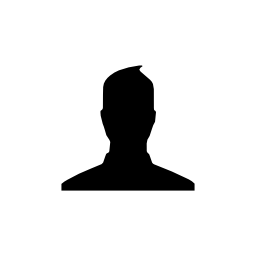
\includegraphics[scale=0.2]{img/fbuser.png}}
                (0,0) node [block] (fb) {
\includegraphics[scale=0.10]{img/fb_icon.png}}
                (5.5, 0) node [block] (friends) {
\includegraphics[scale=0.3]{img/fbfriends.png}}

                %Top part (PKG lists)
                (-3,4) node [block] (linkedin) {
\includegraphics[scale=0.1]{img/linkedin.png}}
                (-4,5) node [block] (fbpkg) {
\includegraphics[scale=0.06]{img/fb_icon.png}}
                (1.2,5) node [block] (gplus) {
\includegraphics[scale=0.08]{img/gplus.png}}
                (-2,5.2) node [block] (tumblr) {
\includegraphics[scale=0.1]{img/tumblr.png}}
                (2.8,4) node [block] (pin) {
\includegraphics[scale=0.05]{img/pinterest.png}}
                (4.2,5) node [block] (tor) {
\includegraphics[scale=0.1]{img/tor.png}}
                (-0.5,4) node [block] (twitter) {
\includegraphics[scale=0.05]{img/twitter.png}};

            \node[below=of fb] {\textbf{Facebook}};
            \node[below=of user] {\textbf{Gebruiker}};
            \node[below=of friends] (frdcaption) {\textbf{Deelverzameling van gewenste ontvangers}};
            \node[below=of frdcaption] {\textbf{zodat, $\mathcal{S}=\{\id{1},\id{2},\ldots,\id{\eta}\}$}};


            \begin{scope}[every path/.style=line]
                \path (user.east) -- (fb.west);               
            \end{scope}   

            % Legend
            \path (-2.8,0.35) node [leg] {Publiceer: $C\leftarrow$ Encrypteer($m$,$\mathcal{S}$)};
            \path (2.7,0.35) node [leg] {Download $C$};
            \node[right=of friends] {Decrypteer($C$)};
                
            \begin{scope}[every path/.style=line2]
                \path (fb) -- (friends);
                \path[dashed] (friends.north) -- (tor.south);
                \path[dashed] (5.1,1) -- (3.1,3.4);
                \path[dashed] (4.7,0.95) -- (0.5,3.5);
            \end{scope}
        \end{tikzpicture}
    }
    \end{center}
    \caption{Overzicht van een opstelling waarin meerdere OSNen een $(n,t)$-gedistribueerd publiek sleutel protocol aanbieden op basis van identiteitsgebaseerde encryptie. Een bericht $m$ wordt gepubliceerd op Facebook voor een deelverzameling $\mathcal{S}$ van ontvangers voor $t=3$. Het gedistribueerd sleutel protocol kan door elke organisatie ondersteund worden met een motivatie om de privacy op sociale netwerken te waarborgen.}
    \label{fig:overzicht}
\end{figure}

Figuur~\ref{fig:overzicht} toont een mogelijke opstelling in dewelke OSNen zelf de ondersteuning van de publieke sleutel generatoren verzorgen. Indien OSNen collectief hun gebruikersaantal zien dalen omwille van een slechte privacy policy, kan het een motivatie zijn om een dergelijke infrastructuur aan te bieden. Zeker in het kader van recente bekendmakingen van Edward Snowden over het spionageprogramma van de NSA, hebben OSNen elke motivatie om hun data te beschermen. Hoewel de OSNen bij een dergelijke opstelling geen gerichte reclame meer kunnen aanbieden, hebben ze er alle baat bij dat hun totaal gebruikersaantal niet verder afneemt. Doordat nooit meer dan $t$ rivaliserende OSN providers geneigd zijn om hun deel van de private sleutel bekend te maken, wordt de veiligheid van de opstelling gegarandeerd. Bemerk dat de publieke sleutel generatoren ook ondersteund kunnen worden door gesubsidieerde onderzoeksinstellingen of verschillende overheden.

Ge{\"i}nspireerd door het voorgaande, werken we aan de hand van identiteitsgebaseerde encryptie een algoritme uit dat toelaat om versleutelde informatie te delen met meerdere gebruikers zonder hun identiteit aan de buitenwereld te onthullen. De oplossing laat toe om versleutelde informatie te versturen aan gebruikers die nog niet expliciet hebben ingetekend om deel uit te maken van een dergelijke infrastructuur. Ten slotte, tonen we de haalbaarheid van onze oplossing aan door een open-source prototype te ontwikkelen dat praktisch bruikbaar is op Facebook en eenvoudig te veralgemenen valt naar andere bestaande OSNen.


%%% Local Variables: 
%%% mode: latex
%%% TeX-master: "thesis"
%%% End: 

\chapter{English Paper}
\label{app:english_paper}

%%% Local Variables: 
%%% mode: latex
%%% TeX-master: "thesis"
%%% End: 


\backmatter
% The bibliography comes after the appendices.
% You can replace the standard "abbrv" bibliography style by another one.
\bibliographystyle{abbrv}
\bibliography{references}

\end{document}

%%% Local Variables: 
%%% mode: latex
%%% TeX-master: t
%%% End: 
